\documentclass{apuntes}

\usepackage{tikztools}
\usepackage{tikz-3dplot}
\usepackage{textcomp}
\usepackage{tikz-qtree}
% subfiguras
\usetikzlibrary{arrows}

\newcommand{\theauthor}{}
\newcommand{\thetitle}{Modelización\\ Porque los apuntes de Chamizo son demasiado fáciles}
\newcommand{\rightheader}{Modelización}
\newcommand{\leftheader}{UAM - 2014/2015}

% Si no compila y el directorio tikzgen está creado, quitar estas dos sentencias.
%\precompileImages
%\precompileTikz

\title{Modelización}
\author{Guillermo Guridi Mateos\\Cristina Kasner Toruné}
\date{Curso 2014 - 2015 C2}

% Paquetes adicionales

% --------------------

\newcommand{\cte}{\text{Cte}}

\begin{document}
\pagestyle{plain}
\maketitle
%\abstract{Porque los apuntes de Chamizo son demasiado fáciles}

\tableofcontents
\newpage
% Contenido.

\chapter{Introducción}

\section{¿De qué trata la modelización?}

La modelización trata de dar descripciones de sistemas (situaciones) reales con un lenguaje matemático. Resulta particularmente útil en Física.

Entre los siglos XVII y XVIII se compilaban tablas astronómicas muy precisas con medidas acerca de los ángulos con los que podía verse cada planeta en un instante determinado. Las tablas más precisas fueron creadas por Tycho Brahe y eran realmente codiciadas por Kepler.

Kepler desarrolló un modelo matemático que sostenía, entre otras cosas, que los planetas se movían en elipses. Kepler estaba muy interesado en obtener las tablas de Tycho Brahe pues quería analizarlas con el fin de poder probar sus teorías. Finalmente, con la muerte de su creador, Kepler las heredó y pudo establecer una relación entre los cuadrados de los períodos y el cubo de los radios de giro de los planteas.

Posteriormente llegó Newton, que modelizó el movimiento de los planetas con la fórmula:

$$F = - \frac{GMm}{r^2}$$

Esta fórmula en su momento tuvo una gran importancia filosófica, pues permitía explicar toda la teoría acerca del movimiento de los planetas a partir de una ecuación muy simple. No obstante, la utilidad matemático-física de esta ecuación en el momento de su descubrimiento era prácticamente nula.

Newton no conocía el valor de G y si consideramos las interacciones entre los planetas la fórmula se complica mucho. Sin embargo, esta fórmula seguía (y sigue) suponiendo una aproximación bastante acertada.

Así funciona la modelización, a partir de datos surge una idea o explicación matemática que más tarde es complementada con un modelo matemático.


\chapter{Gravitación y leyes de kepler}
\section{Leyes de Kepler}

Kepler, a principios del siglo XVII, enunció unas leyes experimentales (con datos de Tycho Brahe):

\begin{lemma}[1ª Ley de Kepler]
	Las órbitas de los planetas son elipses con el Sol en uno de los focos.
\end{lemma}

\begin{lemma}[2ª Ley de Kepler]
	La linea que une un planeta y el Sol barre áreas iguales en tiempos iguales.
\end{lemma}

\begin{lemma}[3ª Ley de Kepler]
	El cuadrado del periodo orbital es proporcional al cubo del semieje mayor de la órbita.
\end{lemma}

\section{Newton}

Gracias a Newton, en 1985, las leyes de Kepler pudieron demostrarse matemáticamente suponiendo que la fuerza gravitacional obedece la ecuación
\[ F = \frac{-GMm}{r^2} \]
en la dirección del vector radio.

No existe una forma sencilla de realizar esta demostración a menos que demos por sentados muchos principios físicos que no eran conocidos en aquella época. Vamos a tratar de realizar la demostración utilizando los mínimos ``trucos'' posibles.

Para empezar debemos recordar que toda fuerza puede calcularse como:
$$ \overrightarrow{F} = m\ga$$

La aceleración se calcula a partir de la posición de una partícula, que viene dada por: $\vr = (x(t), y(t), z(t))$. La aceleración se define como la derivada segunda de la posición con respecto al tiempo. Es decir:
\[ \ga = \frac{d^2\vr}{d t^2} \]

Esta fórmula describe, por ejemplo, la atracción que ejerce el Sol sobre la Tierra, por ello el signo negativo. En el caso de el Sol y la Tierra, la fuerza recíproca no se tiene en cuenta ya que el Sol es demasiado pesado como para ser influido apreciablemente por la gravedad de la Tierra. Hay que hacer mediciones muy finas para poder detectar estas perturbaciones.

Para poder seguir con la demostración de forma relativamente sencilla, \textbf{despreciamos la fuerza de los planetas sobre el Sol y de los planetas entre ellos.}

Por lo tanto, modelamos tomando sólo un planeta y asumiendo un Sol fijo.

Igualando las dós fórmulas para el cálculo de la fuerza que hemos indicado, obtenemos:

$$ \frac{-GMm}{{||r||}^2} \frac{\vr}{{||r||}^2}  =  m \frac{d^2\vr}{d t^2}$$


En primer lugar vamos a probar que las soluciones $\vr = \vr(t)$ de esta ecuación diferencial satisfacen las leyes de Kepler (con las condiciones iniciales de los planetas)

%Esto es un sistema con una llave
$$
\begin{cases}
 x'' = \frac{-GMx}{(x^2 + y^2 + z^2)^{3/2}}\\
 y'' = \frac{-GMy}{(x^2 + y^2 + z^2)^{3/2}}\\
 z'' = \frac{-GMz}{(x^2 + y^2 + z^2)^{3/2}}\\
\end{cases}
$$


 \begin{obs}
 No se pueden calcular explícitamente $x$, $y$ y $z$, en función de $t$. $\vr = \vr(t)$ no tiene una fórmula cerrada (en términos de funciones elementales\footnote{Las de la calculadora (sin, cos...)}). Aun así se puede demostrar que la fórmula es una elipse.
 \end{obs}


 %Un método es un truco que sirve varias veces
Vamos a probar que la curva $\vr = \vr(t)$ está contenida en un plano.

Un posible método es usar que una curva es plana si y sólo $τ \equiv 0$, donde τ es la torsión de la curva. Dicha fórmula involucra un determinante con una fila $r$ y otra $r''$, como son proporcionales, la torsión sale 0.


Nuestro método más sencillo se basa en tomar $\overrightarrow{L}(t) = \vr(x) \times \frac{d\vr}{dt}$.

Derivando obtenemos:
$$\frac{d\overrightarrow{L}(t)}{dt} = \frac{d\vr}{dt} \times \frac{d\vr}{dt} + \vr(t) + \frac{d^2\vr}{dt^2} = \overrightarrow{0}$$

de donde podemos deducir que $\overrightarrow{L}$ es un vector constante $\Rightarrow \vr \perp \overrightarrow{L} \Rightarrow \vr(t)$ está contenida en el plano $\overrightarrow{L}(x,y,z) = 0 $.
(pensar $\overrightarrow{L} = \overrightarrow{0}$).

Por comodidad, vamos a girar el plano en que se encuentra la órbita del planeta, $\vr \rightarrow G\vr$, siengo G un giro (matriz ortogonal), para convertirlo en el plano $z=0$.

Podemos comprobar que este giro no afecta a las cuentas puesto que, en definitiva, estamos multiplicando por una constante.

$$\frac{d^2\vr}{dt^2} = \text{cte}\frac{\vr}{||\vr||^3} \Leftrightarrow \frac{d^2(G\vr)}{dt^2} = \text{cte}\frac{G\vr}{||G\vr||^3}$$

En definitiva "girando la cabeza" (aplicando el cambio $\vr \rightarrow G\vr$) podemos suponer que la curva $\vr = \vr(t)$ está contenida en el plano $z = 0$, así que simplemente supondremos que $z(t) = 0$. El sistema nos quedaría así:


%Esto es un sistema con una llave
$$
\begin{cases}
 x'' = k\frac{x}{(x^2 + y^2)^{3/2}}\\
 y'' = k\frac{y}{(x^2 + y^2)^{3/2}}\\
\end{cases}
$$

\subsection{Demostración de las leyes de Kepler}

Vamos a probar las leyes de Kepler para $t \rightarrow (x(t), y(t))$ utilizando los resultados de Newton.

La forma de la solución será una elipse.
Si escribimos $x$ e $y$ en polares, el sistema nos quedará más sencillo.

% % align, gather y equation.
$$\begin{array}{c}
x = r\cos(\theta)\\
y = r\sin(\theta) \\
r = r(t) \\
\theta = \theta(t)
\end{array}
$$

(r y $\theta$ no se pueden calcular eplícitamente.)

Y con esto sacamos las ecuaciones de gravitación:
\begin{gather}
r''\cos\theta - 2r'\theta'\sin\theta - r(\theta')^2\cos\theta - r\theta''\sin\theta = cte \frac{\cos\theta}{r^2} \label{eq1_kepler}\\
r''\sin\theta + 2r'\theta'\cos\theta - r(\theta')^2\sin\theta + r\theta''\cos\theta = cte \frac{\sin\theta}{r^2} \label{eq2_kepler}
\end{gather}
$\eqref{eq1_kepler}\cdot\cos\theta + \eqref{eq2_kepler}\cdot\sin\theta \rightarrow K= r^3(\theta')^2 - r^2*r'' \rightarrow$ 1ª ecuación de gravitación
$$-\eqref{eq1_kepler}\cdot\sin\theta + \eqref{eq2_kepler}\cdot\cos\theta \rightarrow 0= r \theta'' + 2r' * \theta' \rightarrow \text{2ª ecuación de gravitación}$$


\subsubsection{2ª ley de Kepler}
\paragraph{Recordemos:}
2ª ley de Kepler : Un planeta recorre áreas iguales en tiempos iguales.

Vamos a estudiar cual es la fórmula para el área.
Primero nos vamos al caso general, para cualquier curva que tengamos en polares.

En este caso el radio depende de $\theta$ \\
Cogemos una curva R.\\

$$A(R) = \int\int_R 1 \dif x \dif y = \int_0^{\theta_0} \int_0^r(\theta) r \dif r \dif \theta = 1/2 \int_0^{\theta_0} r^2(\theta) \dif\theta$$

La idea es coger pequeños triángulos e ir calculando su área

En el caso de la \textbf{ley de Kepler}, si en el tiempo t=0 estamos en $\theta = 0$ y en el tiempo T estamos en $\theta_0 \implies$ la fórmula para el área en función de T sería:

$$A(T) = \frac{1}{2} \int_1^T r^2(t) \theta'(t) \dif t$$


de donde podemos deducir que $\frac {\dif A(T)}{\dif T} = cte$

Es lo mismo que decir $A(T)$ es lineal (a tiempos iguales tengo áreas iguales)

\[A(x + T) - A(x) = A(T) - A(0)\]

Vamos a traducir la 2ª ley de Kepler en algo más familiar (derivadas):

\[\frac{\dif A}{\dif T} = cte \iff r^2\theta' = cte  \text{ (no depende de T) }\]
que puede verse como la conservación del momento angular

Además, $r^2\theta' = cte  \implies (r^2\theta')' = 0 \iff 2rr'\theta' + r²\theta'' =0$ con lo que obtenemos la 2ª ecuación de gravitación.

Por tanto, queda probada la 2ª ley de Kepler.

\subsubsection{1ª ley de Kepler}
Ahora vamos a intentar manipular la 1ª ecuación para probar la \textbf{1ª ley de Kepler} (las óbitas de los planetas son elipses).

Escribimos:
\[h= r^2\theta'=cte \text{ (para cada planeta, } h \text{ es diferente)}\]

1ª ecuación de gravitación:
\[K= r^3(\theta')^2 -r^2*r''\]

como $h = r^2*\theta'$ podemos eliminar $\theta'$ en la 1ªecuación, obteniendo:

$$K= r^3 \frac{h^2}{r^4} - r^2*r''$$
y, simplificando, llegamos a:
$$K= \frac{h^2}{r} - r^2*r''  \rightarrow  \text{Es una EDO ($r = r(t)$) y no aparece explícitamente la t.}$$

\obs En el curso de EDO se ven métodos para pasar de 2 orden ($r''$) a 1 orden ($r$) y se podría expresar r en términos de la imagen inversa de una integral, pero no se puede calcular en términos elementales.

Para resolver la ecuación debemos estar hábiles y realizar un cambio de variable adecuado. En este caso, el cambio de variable consistirá en escribir $r=r(\theta)$ en vez de $r=r(t)$

Hacemos el siguiente cambio de variable:
$$U(\theta(t)) = \frac{1}{r(t)} \implies U'\theta' = \frac{-r}{r^2} \stackrel{h=r^2\theta' }{\iff} hU' = -r' \stackrel{U(\theta(t))}{\implies} hU''\theta' = -r''$$

Sustituyendo en la EDO:

$$K= h^2U + h^2U'' \rightarrow \text{ecuación del movimiento armónico simple}$$
viendo que $\cos'' = -\cos$ y $\sin'' = -\sin$:

$$U'' + U = \frac{K}{h^2} \implies U= \frac{K}{h^2} + \lambda\cos\theta + \mu\sin\theta \iff U= \frac{K}{h^2} + A\cos(\theta - \theta_0)$$
\begin{mdframed}
\obs Al último resultado hemos llegado utilizando que
$$ \lambda\cos\theta + \mu\sin\theta = \sqrt{\lambda^2 + \mu^2}\left(\frac{\lambda}{\sqrt{\lambda^2 + \mu^2}}\cos\theta  +\frac{\mu}{ \sqrt{\lambda^2 + \mu^2}}\sin\theta\right)$$
LLamamos $\cos\theta_0$ a $\frac{\lambda}{ \sqrt{\lambda^2 + \mu^2}}$ y $\sin\theta_0$ a $\frac{\mu}{ \sqrt{\lambda^2 + \mu^2}}$ ya que ambos están entre 0 y 1.
Nos queda que
$$\lambda\cos\theta + \mu\sin\theta = \sqrt{\lambda^2 + \mu^2}(\cos\theta_0\cos\theta + \sin\theta_0\sin\theta) \stackrel{A=\sqrt{\lambda^2 + \mu^2}}{=} A\cos(\theta - \theta_0)$$
\end{mdframed}
Con un giro podemos suponer $\theta_0 = 0$, porque un giro en polares no es más que sumarle una constante al ángulo ($\theta \rightarrow \theta + cte$)

Volviendo al cambio de variable inicial, tenemos
\[U = \frac{1}{r} \implies r=\frac{h^2/K}{1 + B\cos\theta}\]

\textbf{Hecho matemático:} La ecuación general de una cónica en coordenadas polares centradas en un foco con la "orientación habitual" es:

$$r(\theta) = \frac{l}{1+e\cos\theta} \rightarrow
\begin{cases}
l>0\\
e\text{ (excentricidad) }\ge0\\
\end{cases}
$$

\textbf{Recordemos:}

$$\text{excentricidad} \rightarrow
\begin{cases}
0 \le e \le 1 \rightarrow \text{elipse , caso particular} (e=0) \rightarrow \text{circunferencia}\\
e>1 \rightarrow \text{hipérbola(masas no capturadas por el sol)}\\
e=0 \rightarrow \text{parábola}
\end{cases}
$$
Los \textbf{datos astronómicos} para los planetas(excepto mercurio) muestran $B<0.1$ por lo tanto las órbitas son elipses(1ª ley de Kepler) y parecidas a circunferencias.

\begin{center}
\begin{tabular}{| c | c |}
	\hline
	Planetas & B \\
	\hline
	Tierra & 0.016 \\
	\hline
	Venus & 0.0067 \\
	\hline
	Mercurio & 0.20\\
	\hline
\end{tabular}
\end{center}


\subsubsection{3ª ley de Kepler}
%(Dibujo de la elipse con los ejes)
Tomamos $a$ como el semieje mayor y $b$ como semieje menor de la elipse de forma que:
$$2a = \frac{l}{1+e} + \frac{l}{1-e} \implies a= \frac{l}{1-e^2}$$
y
$$b = \sqrt{al}$$
Ahora vamos a calcular área de la elipse basándonos en la fórmula conocida para el área de la circunferencia.

Escribimos la circunferencia como
\[\frac{x^2}{a^2} + \frac{y^2}{a^2} = 1\]
y su área es
\[\pi a^2\]

Si hacemos en cambio de
\[y \rightarrow \frac{a}{b}y\]
nos queda
\[\frac{x^2}{a^2} + \frac{y^2}{b^2} = 1\]
que es la fórmula de la elipse. Por tanto, el área de la elipse será $\pi ab$.

Ahora calculamos el área de la órbita del planeta:
$$T_o = \text{periodo orbital}$$

$$r= \frac{h^2/K}{1 + B\cos\theta}$$

$$\text{Área de la órbita} = A(T_0) = 1/2 \int_0^{T_0} \underbrace{r^2(t)\theta'(t)}_{\text{h}}\dif t = 1/2hT_0$$

Igualando el área de la órbita con  el área de la elipse tenemos:
$$\frac{1}{2}hT_0 = \pi ab= \pi a \sqrt{al} = \pi a\sqrt{a\frac{h^2}{K}} \implies T_0 = cte*a^{3/2}$$
Y queda demostrada la 3ª ley de Kepler.

\obs Para las demostrciones de las tres leyes, en física se ayudan de dos teoremas:
\begin{enumerate}
\item\textbf{Conservación del momento angular}:
$\overrightarrow{L}$ es cte siendo:
\[\overrightarrow{L} = \overrightarrow{r} \times m \overrightarrow{v} (\overrightarrow{r} \rightarrow  \text{ posición },  \overrightarrow{v} \rightarrow \text{ velocidad}).\]


\item\textbf{Conservación de la energía}:\\
\[\frac{1}{2}m||\overrightarrow{v}||^2 + \frac{GMm}{||\overrightarrow{r}||} \rightarrow \text{ es cte}.\]
\end{enumerate}

\subsection{El cabo suelto de Newton}
A Newton le quedó un cabo suelto que vamos a intentar resolver:

\begin{figure}[hbtp]
	\centering
	\inputtikz{ProblemaFGravitacion}
	\caption{¿Se cumple $\md\vf = \frac{GMm}{r^2}$ ?}
\end{figure}
Vemos que en la fórmula, cuando $r \rightarrow 0 \implies \vf \rightarrow \infty$ y esto , en el caso del dibujo, no es real.

Si una masa M está compuesta por varias masas con densidad constante, $\md\vf = \frac{GMm}{r^2}$, con $r =$distancia al punto medio puede cumplirse.

El problema es ver cómo se comporta $\vf$ cuando la densidad de M no es constante.......\\
(.......)\\
Aqui va razonamiento que no he entendido bien y que me va a explicar Miguel cuando pueda.
El caso es que puedo intentar calcular la fuerza que ejerce el Sol sobre la Tierra igual que si fuera sobre una partícula con densidad uniforme.\\
\newpage
\begin{figure}[hbtp]
\centering
\inputtikz{KasnerNoSabePonerNombresANada}
\caption{Divido la esfera con masa M en pequefas particulas $\partial M$}
\label{figaaa}
\end{figure}

Entonces para ver si $\md\vf = \frac{GMm}{r^2}$  es válida, habrá que calcular una integral triple complicada y ver el efecto que tiene en cada partícula.
$$\int\frac{-Gm\overrightarrow{x}}{\md {\overrightarrow{x}}^3}\dif M$$

Hay una manera de calcular esta integral y probar que  $\md{\overrightarrow{\vf}}$ es válida para objetos con simetría esférica, usando el teorema de la divergencia:

\begin{prop}[Ley de Gauss]
	Dada una región sólida B y un campo $\overrightarrow{E} = \frac{\overrightarrow{x}}{\md {\overrightarrow{x}}^3}$ tenemos que:
	\[\int_{\partial B} \overrightarrow E \dif \overrightarrow S =
	\left\{ \begin{array}{lcc}
	     4\pi & si & \overrightarrow 0 \in Int(B) \\
	  \\ 0 & si & \overrightarrow 0 \notin Int(B)
	\end{array} \right.\]
	Siendo $\partial B$ la frontera de B
\end{prop}
\begin{proof}
	\begin{itemize}
	\item Si $\overrightarrow 0$ está fuera de B, el campo $\overrightarrow E$ es regular ($C^{\infty}$) en B.\\
	$$\int_{\partial B} \overrightarrow E \dif \overrightarrow S \stackrel{Tª divergencia}{=} \int_B div \overrightarrow E = 0$$

	\item Si $\overrightarrow 0$ pertenece a Int(B):\\
	En lugar de B consideramos $B - B_{\delta}$ con $B_{\delta} = \{ \md{\overrightarrow x} \le \delta \} $\\
	$$\overline{B} = B- B_\delta \rightarrow \int_{\partial {\overline{B}}} \overrightarrow E \dif \overrightarrow S = \int_B div \overrightarrow E = 0$$
	Como $\partial{\overline{B}} = \partial B \cup \partial{B_\delta}$ con orientaciones distintas $\rightarrow$ $$ \int_{\partial B} \overrightarrow E \dif \overrightarrow S - \int _{\partial{B_\delta}} \overrightarrow E \dif \overrightarrow S = 0$$
	$$ \int_{\partial B} \overrightarrow E \dif \overrightarrow S = \int _{\partial{B_\delta}} \overrightarrow E \dif \overrightarrow S \overbrace{=}^{esfericas} \int_0^{\pi} \int_0^{2\pi} \frac{\delta ^2 \sin\theta}{\delta ^3} \delta \dif \phi \dif \theta = 4\pi$$
	\end{itemize}
\end{proof}
\newpage
Por lo tanto, tenemos que:

\begin{figure}[hbtp]
	\centering
	\inputtikz{ProbGravitacion2}
	\caption{No hace falta que B y B' sean regulares, pero aún no se dibujar otra cosa}
\end{figure}
$$\overrightarrow F = - \frac{GMm}{\md{\overrightarrow x - \overrightarrow y}}(\overrightarrow x - \overrightarrow y)$$
 Si $\overrightarrow y $ se mueve en $B'$
 $$\int_{\partial B} \overrightarrow F \dif \overrightarrow S =
 \begin{cases}
 0\\
 -4\pi GMm\\
 \end{cases}
 \rightarrow \text{Dependiendo de si} \overrightarrow x \text{está fuera o dentro de B'}$$

 Si tenemos muchas masas, también es cierta la proposición.\\

\begin{figure}[hbtp]
	\centering
	\inputtikz{ProbGravitacion3}
	\caption{$\int_{\partial B} \vf \dif \vec{S} = -4\pi GMm $ Con M suma de las m en el interior}
\end{figure}
\newpage
\paragraph{Conclusión}
En el caso de los planetas, $\overrightarrow F$ tiene que ser una función radial (por la simetría de la esfera), si cogemos B una "esfera ficticia" de radio $r = \md{\overrightarrow y} \implies$
\begin{figure}[hbtp]
	\centering
	\inputtikz{ProbGravitacion4}
\end{figure}
$$\int_{\partial B} \overrightarrow F \dif \overrightarrow S = 4 \pi r^2 |\overrightarrow F|$$
Como $\int_{\partial B} \overrightarrow F \dif \overrightarrow S = -4\pi GMm  \implies$
$$ - 4\pi r^2 |\overrightarrow F| = -4\pi GMm \implies |\overrightarrow F| = \frac{GMm}{r^2}$$

Por lo tanto, $|\overrightarrow F| = \frac{GMm}{r^2}$ , que es la fórmula de Newton, es válida con objetos con simetría radial y por lo tanto válida para los planetas.



\subsection{Un poco de mecánica analítica}
Lagrange escribió un libro llamado "Mecánica Analítica" publicado en 1788. Este libro describía la mecánica de manera muy matemática. Entre sus ventajas estaba la unificación de la mecánica. Todo se regía en base a un principio con adición de teoremas y era muy matemático. Además la mecánica sufrio una simplificación, como por ejemplo la libretad para escoger las coordenadas libremente.

\begin{prop}[Cálculo de variaciones]
Dada L regular de $2n + 1$ variables. Supongamos que la integral:

 $$\int_a^b L(q_1(t),...,q_n(t),\dot{q_1}(t),...,\dot{q_n}(t),t) dt$$

 (donde $\dot{q_i} = \frac{dq_i}{dt}$.)

 alcanza un máximo o mínimo para ciertas $q_i 1\leq i \leq n$ regulares con valores $q_i(a)$, $q_i(b)$ fijados. Entonces dichas $q_i$ satisfacen:


\begin{op}{Ecuaciones de Euler-Lagrange}
 \frac{d}{dt}(\frac{\sigma L}{\sigma \dot{q_i}}) = \frac{\sigma L}{\sigma q_i}    1 \leq i \leq n
\end{op}

Además si L no depende de la última variable (la t suelta) la energúa $ E = \sum_{i=1}^n \dot{q_i} \frac{\sigma L}{\sigma \dot{q_i}} - L$ es constante para las $q_i$ solución.

Las propiedades minimizantes o maximizantes no dependen de las coordenadas elegidas (polares, cartesianas, etc…).

\end{prop}

En los  siguientes ejemplos damos por supuesto la existencia:

\begin{example}
Hallar la curva $\sigma (t) = (t, y(t))$ más corta que conecta $(0,0)$ y $(1,1)$.

(FIGURA)

$$ \text{longitud} = \int_0^1 || \sigma'(t) || dt = \int_0^1 \sqrt{1 + (y'(t))^2} dt$$

$$y = q \; y' = \dot{q} \; n=1 \; L = \sqrt{1 + \dot{q}^2}$$

Pasamos a las ecuaciones de Euler-Lagrange:

$$\frac{d}{dt}(\frac{\sigma L}{\sigma \dot{q}}) = \frac{\sigma L}{\sigma q} \; \frac{d}{dt}(\frac{2 \dot{q}}{2 \sqrt{1 + \dot{q}^2}}) = 0$$

$$\Rightarrow \frac{q}{\sqrt{1 + \dot{q}^2}} = \text{cte} \Rightarrow \frac{\dot{q}^2}{1 + \dot{q}^2} = \text{cte} \Rightarrow \dot{q} = \text{cte} \Rightarrow q(t) = At + B $$

$$ y = 1 \; q(0) = 0 \; q(1) = 1 \Rightarrow q(t) = y(t) = t \Rightarrow \sigma (t) = (t,t) \text(una recta)$$

\begin{obs}
$$E = \dot{q} \frac{\sigma L}{\sigma \dot{q}} - L \Rightarrow \text{cte} = \dot{q} \frac{\dot{q}}{\sqrt{1 + \dot{q}^2}} - \sqrt{1 + \dot{q}^2} = \frac{-1}{\sqrt{1 + \dot{q}^2}} \Rightarrow \dot{q} = \text{cte}$$
\end{obs}

\end{example}




\begin{example}
(Braquistocrona, J.Bernouilli, Newton, Euler, Lagrange) Hallar el tobogán más rápido que une $(0,0)$ y $(\frac{\pi}{2},-1)$.

FIGURA

h = altura medida desde el origen.

Vamos a parametrizar la curva en función de la altura. Ponemos la x en función de la y.


En mecánica la velocidad vertical viene dada por:

$$\frac{dh}{dt} = \frac{\sqrt{2gh}}{\sqrt{1+(x'(h))^2}}$$

Para calcular el tiempo total integramos:

$$\int_0^1 \frac{dt}{dh} dh = \int_0^1 \frac{\sqrt{1 + (x')^2}}{\sqrt{2gh}} dh \;\; g = 9.8$$

$$ n=1 \; t=h \; q=x \;  \dot{q}=x' \; L = \frac{\sqrt{1+\dot{q}^2}}{\sqrt{2gt}} $$


%Aquí hay un = 0 encima de la fracción \frac{\sigma L}{\sigma q}  la primera vez que aparece
$$\frac{d}{dt} (\frac{\sigma L}{\sigma \dot{q}}) = \frac{\sigma L}{\sigma q} \; \frac{\sigma L}{\sigma \dot{q}} = \text{cte} \Rightarrow \frac{\dot{q}}{\sqrt{t(1+\dot{q}^2)}} = \text{cte}$$

$$ \Rightarrow^{\text{EDO (un poco dificil)}} q(t) = \frac{u - \sin(u)}{2} \; t \sin^2(\frac{u}{2}) $$

$$ \Rightarrow \text{Tobogán:} \sigma (u) = ( \frac{u - \sin{u}}{2}, -\sin^2(\frac{u}{2}) ) $$

(Figura cicloide)




\end{example}





\chapter{Cadenas de Markov}

\section{Un modelo para redes}
En este capítulo vamos a ver cómo ordena Google las páginas que resultan de la búsqueda para mostrarlas por orden de prioridad.

Supongamos que tenemos una red de páginas web conectadas por enlaces (Google afirma cubrir unas $3\cdot 10^{13}$ páginas web). Vamos a ver las páginas como vértices de un grafo y los enlaces como aristas dirigidas(especificando un sentido).

Matemáticamente esto es un grafo dirigido:
\begin{center}
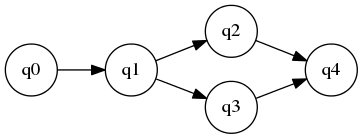
\includegraphics{tex/ejemplo_dibujo.png}
\end{center}
¿Cómo ordenar por relevancia los vértices?¿En qué orden aparecerán las páginas?


Para poder determinar qué páginas son más importantes vamos a suponer un paseo aleatorio por los vértices (los internautas navegan al azar siguiendo los enlaces) de forma que una mayor acumulación en ciertos vértices indicará que son más importantes.


\obs No funciona literalmente, hay que hacer modificaciones.

A la larga esto converge...
\begin{center}
	\centering
	\inputtikz{grafos_mod}
\end{center}




Como había 360 al principio parece que:


\begin{itemize}
	\item Probabilidad de estar en 1 es $\frac{144}{360} = \frac{2}{5}$
	\item Probabilidad de estar en 2 es $\frac{144}{360} = \frac{2}{5}$
	\item Probabilidad de estar en 3 es $\frac{72}{360} = \frac{1}{5}$
\end{itemize}
	Según esto 1 y 2 son igual de importantes y 3 es la mitad de importante.

	La distribución que pensamos que da el límite es estacionaria (no cambia con el tiempo).



% Empieza clase del 4 de Febrero

Recordamos que en la red anterior cuando el tiempo tiende a infinito parece que la distribución de personas se estabiliza.


Parece además que sea cual sea la distribución inicial llegamos a proporciones similares. En este caso llegamos a la distribución límite $\left(\frac{2}{5},\frac{2}{5},\frac{1}{5}\right)$, que es una distribución estacionaria (no varía con el tiempo).

\section{Propiedades de los paseos aleatorios}

\textbf{¿Esta simulación con paseos aleatorios siempre sirve para ordenar los vértices (páginas web)?}

Debemos estudiar las siguientes preguntas:

\begin{itemize}
	\item ¿Existe siempre una distribución estacionaria?
	\item Si existe una distribución estacionaria ¿es única?
	\item El procedimiento, ¿Da lugar siempre a una distribución límite?
	\item Si la distribución límite existe, ¿es independiente de la distribución inicial?

\end{itemize}

Vamos a analizar estas preguntas y sus respuestas una a una.

\subsection{Si existe una distribución estacionaria ¿es única?}
\label{P2}

\begin{center}
	\centering
	\inputtikz{grafosIncomunicados}
\end{center}
% nodo 4 es internet oscura

Como desde un lado de la red no se puede acceder al otro podemos decir que las  distribuciones $(\frac{2}{5},\frac{2}{5},\frac{1}{5}, 0, 0 , 0, 0)$ y $(0, 0, 0, 0, \frac{1}{5}, \frac{2}{5}, \frac{2}{5})$ son estacionarias:

\subsection{¿Existe siempre una distribución estacionaria?}

\begin{example}{Sencillo}

	\begin{center}
		\centering
		\inputtikz{grafo3nodosSimpleTik}
	\end{center}

	Si pones todos en un nodo oscila:

	$1\; 0\; 0 \rightarrow 0\; 0\; 1 \rightarrow 0\; 1\; 0 \rightarrow 1\; 0\; 0$

	Se puede argumentar que con una distribución inicial uniforme si funciona:

	$\frac{1}{3} \; \frac{1}{3} \; \frac{1}{3} \; \rightarrow \frac{1}{3} \; \frac{1}{3} \; \frac{1}{3} \; $

	Pero esto no es verdad para cualquier grafo: partiendo de la equidistribución no se tiene la convergencia en general.

	\begin{center}
		\centering
		\inputtikz{grafo4nodosTik}
	\end{center}


	$(\frac{1}{4},\frac{1}{4},\frac{1}{4},\frac{1}{4}) \rightarrow (\frac{1}{2},\frac{1}{4},\frac{1}{4}, 0) \rightarrow (\frac{1}{4},\frac{1}{4},\frac{1}{2},0)$ oscila como antes

	\textbf{La respuesta es negativa en general}

\end{example}

\subsection {¿Existe siempre una distribución límite?}
El mismo ejemplo del apartado anterior nos sirve para ver claramente que no es así. Según que distribución inicial escojamos podemos llegar a encontrarnos con un caso sin distribución límite.

\subsection {Si la distribución límite existe, ¿Es independiente de la distribución inicial?}


Basta usar como distribución inicial las distribuciones estacionarias que vimos para la segunda pregunta \ref{P2}.

\begin{obs}

Para el grafo de \ref{P2} se puede probar que $\exists$ límite:

$$(1-t)\left(\frac{2}{5},\frac{2}{5},\frac{1}{5},0,0,0,0\right) + t \left(0,0,0,0,\frac{1}{5},\frac{2}{5},\frac{2}{5}\right) \;\;\; 0 \leq t \leq 1 $$

son infinitos contraejemplos como los necesarios para la segunda pregunta \ref{P2} y la cuarta.

\end{obs}


\textbf{Spoiler} P1 es verdad y "perturbando" un poco el grafo (de manera muy sencilla) todas las preguntas tienen respuesta afirmativa.



\section{Cadenas de Markov}

\begin{defn}[Cadena de markov]
	Es una sucesión de variables aleatorias $\{X_n\}_{n=0}^{\infty}$ que toman valores en un conjunto numerable S (\textbf{conjunto de estados}) tal que
	$$Prob(X_{n+1} = V | X_n = U) = Prob(X_{n+1} = V | X_n =U , X_{n-1} = U_{n-1} , ... , X_0 = U_0)$$
	para cualesquiera $n \geq 0$ $U,V,U_0,.... ,U_{n-1} \in S$
\end{defn}


\obs Además supondremos que esta probabilidad no depende de n.


\textbf{Idea intuitiva: } n es el tiempo discretizado, lo que ocurra mañana depende con cierta probabilidad de lo que ocurre hoy sin que importe conocer la historia anterior.

Decir que no depende de n es decir que según pasa el tiempo, las reglas no cambian.

\begin{example}
	$X_n =$ suma de puntuaciones el día $n$ al tirar un dado cada día.

	El conjunto de todos los estados serían todas las puntuaciones posibles . (S = naturales)

	Sabiendo lo que llevo acumulado hoy, tengo una cierta probabilidad de obtener mañana diferentes resultados, pero no depende de lo que ocurrió ayer; no me importa cómo he llegado a sumar lo que llevo hoy.
\end{example}

\begin{example}[2]
	S = puntuaciones en el tenis.\\
	$X_n =$ puntuación el en punto n\\
	Suponemos que el jugador A tiene prob $p > 1/2$ de ganar cada punto.\\
	Pensando un poco las puntuaciones en el tenis vemos que S solo puede tener 20 elementos.\\
	S= puntuaciones numéricas, deuce, advantages(A o B) , victoria (A o B).\\
	Se puede comprobar que:
	$$Prob(\text{victoria A}) = \frac{p^4 \cdot(1- 16(1-p)^4)}{p^4 - (1-p)^4}$$
	Esto es como curiosidad, ver que con tener sólo un poco más de probabilidad de ganar un punto, la probabilidad de ganar un juego y un set va creciendo.
\end{example}




Si $|S| = \infty$ entonces la cadena de Markov es infinita y se supone $S = \ent^+ (\nat -\{0\})$


Si $|S| < \infty$ entonces la cadena de Markov es finita y se supone $S =\{1,2,...,N\}$

\begin{defn}[Probabilidad de transición]
	del estado i al j
	$$P_{ij} = Prob(X_{n+1} = j| X_n = i) = Prob (X_1 = j| X_0 = i)$$
\end{defn}

Los $P_{ij}$ forman la \textbf{matriz de transición}.

\textbf{Propiedades}
\begin{enumerate}
	\item $\sum_{j \in S} P_{ij} = 1$
	\item $Prob(X_1 = j)= \sum_{i \in S} Prob(X_0 = i)P_{ij}$\\
\end{enumerate}

\begin{proof}
	\begin{enumerate}
		\item $\sum_{j \in S} P_{ij} = \sum_{j\in S} Prob(X_1 = j | X_0 = i) = Prob (X_1 \in S | X_0 = i) = 1$
		\item Utilizando la ley de la probabilidad total

		$$Prob(X_1 = j) = \sum_{i \in S} Prob (X_0 = i) \cdot Prob(X_1 = j| X_0 = i)$$
	\end{enumerate}
\end{proof}

	\begin{defn}[Ley de la probabilidad total]
		Sea  $\{A_1, A_2,...,A_n\}$ una partición de $\Omega$ con $P(A_i)>0 \ \forall i=1,2,...,n$. Entonces, $\forall B \subset \Omega$ medible (perteneciente a $\algb{M}$):
		\[
		P(B)=\sum_{i=1}^{n}P(B\cap A_i)=\sum_{i=1}^{n}P(B|A_i)P(A_i)
		\]
		Esta propiedad se obtiene de despejar de la formula de la probabilidad condicionada:
		\[P(A|B)=\frac{P(A \cap B)}{P(B)}\]
	\end{defn}

\newpage
De las dos propiedades deducimos que:
\begin{itemize}
	\item \textbf{(prop.1)} La matriz de transición $P_{ij} i,j \in S$ tiene elementos $0 \leq P_{ij} \leq 1$ y la suma de los elementos de cada fila es 1.
	\item Escribiendo ($\Pi_0$) = ${Prob (X_0 =i)}_{i \in S}$ como vector fila, y ($\Pi_n$) = ${Prob (X_n =i)}_{i \in S}$

	Entonces por \textbf{(prop.2)} : ($\Pi_1$) $ = (\Pi_0)\cdot P$ (P = matriz de transición)
\end{itemize}

De la misma forma $(\Pi_2) = (\Pi_1) \cdot P$, etc...

Iterando nos queda:
$$\left(\Pi_n\right) = \left(\Pi_0\right) \cdot P^n$$

Ahora vemos cómo aplicar esto a las páginas web.


Teniendo en cuenta que en la realidad la P sería una matriz de $3\cdot 10^{13} \times 3\cdot 10^{13}$ la forma más fácil de calcular $P^n$ es con la forma canónica de Jordan. Veámoslo con un ejemplo.
\begin{example}[1]{}

%Hola kasner, tienes dos opciones, la que creo que quieres es la que no está comentada, q es la que está justo despues de la comentada. Ala, me debes un café.

%\begin{figure}[ht]
%	\centering
%	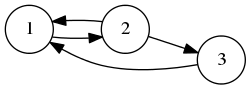
\includegraphics{tex/grafo3nodos.png}
%	\caption{Figurita molona}
%\end{figure}

	\begin{center}
	\centering
	\inputtikz{grafo3nodosTik}
\end{center}


	S= páginas web (vértices)\\
	$P_{ij}$ = probabilidad de , estando en la página i, llegar a la página j en el instante siguiente.

	$$Prob(X_1 = (2)| X_0 = (1)) = 1$$
	$$P =\left(\begin{matrix}
	0 & 1 & 0\\
	1/2 & 0 & 1/2\\
	1 & 0 & 0
	\end{matrix}\right)$$

	Hacemos Jordan:
	$$P = C^{-1} \left(\begin{matrix}
	1&&\\
	&z&\\
	&&\overline{z}
	\end{matrix}\right) C$$
	Haciendo los cálculos nos queda $z = \frac{1}{\sqrt{2}}\cdot e^{\frac{3\pi i}{4}}$

	Por lo tanto:
	$$P^n =  C^{-1} \left(\begin{matrix}
	1&&\\
	&z^n&\\
	&&\overline{z}^n
	\end{matrix}\right) C \stackrel{n\rightarrow \infty}{\rightarrow}  C^{-1} \left(\begin{matrix}
	1&&\\
	&0&\\
	&&0
	\end{matrix}\right) C = \left(\begin{matrix}
	2/5&2/5&1/5\\
	2/5&2/5&1/5\\
	2/5&2/5&1/5
	\end{matrix}\right) = L$$
	Esto implica que:
	$$\lim_{n\rightarrow\infty}\left(\Pi_n\right) = \lim_{n\rightarrow\infty}\left(\Pi_0\right)\cdot P^n = \left(\Pi_0\right)\cdot L =( \begin{matrix}
	2/5&2/5&2/5
	\end{matrix})$$
	Que es independiente de $\Pi_0$
\end{example}

\begin{example}[2]

	\begin{center}
		\centering
		\inputtikz{grafo4nodosTik}
	\end{center}

	$$P = \left( \begin{matrix}
	0 & 1 & 0 & 0\\
	0 & 0 & 1 & 0\\
	1 & 0 & 0 & 0\\
	1 & 0 & 0 & 0\\
	\end{matrix}\right)= C^{-1} \left(\begin{matrix}
	1&&&&\\
	&w&&&\\
	&&\overline{w}&\\
	&&&0
	\end{matrix}
	\right)\cdot C$$
	$w = e^{\frac{2\pi i}{3}}$ , si seguimos calculando las potencias de $w$ y de $\overline{w}$ vemos que van oscilando entre los valores $w , \overline{w} , 1$, por lo que vemos que en este caso $P^n$ no tiene límite.
	$$\exists\left(\Pi_0\right) : \nexists \lim \left(\Pi_0\right)\cdot P^n$$
	Sin embargo con $(\Pi_0) = (\begin{matrix}
	1/3&1/3&1/3&0
	\end{matrix}) $ se comprueba $(\Pi_0) = (\Pi_0)\cdot P$


	Con lo que para ese $(\Pi_0)$ si tenemos límite.Ya veremos más adelante cómo se llaman este tipo de distribuciones.
\end{example}

Lo que hemos comprobado con estos dos ejemplos es que si conocemos la forma canónica de Jordan podemos saber si tenemos convergencia o no.

\paragraph{Resumen de lo visto hasta ahora}
\begin{itemize}
	\item Cadenas de Markov $\begin{cases}
	(\Pi_0) = \{P(X_0 = i)\}_{i \in S} \rightarrow \text{\textbf{distribución inicial}}\\
	P = \text{Matriz de transición}
	\end{cases}$
	\item Distribución de probabilidad en el instante $n = (\Pi_0)P^n$
	\item $P^n$ se calcula con la forma canónica de Jordan
	\item En general queremos que exista la \textbf{distribución límite} : $\lim_{n\rightarrow\infty} (\Pi_0) P^n$
\end{itemize}

\obs Si existe $\left(\Pi\right) = \lim \left(\Pi_0\right) P^n$ entonces $\left(\Pi\right) = \left(\Pi\right) P$
\begin{proof}
	$\left(\Pi\right) = \lim\left(\Pi_0\right) P^{n+1} = \left(\lim \left(\Pi_0\right)P^n\right)P = \left(\Pi\right) P$
\end{proof}

\begin{defn}[Distribuciones estacionarias]
	Se dice que $\left(\Pi\right)$ es una distribución de probabilidad estacionaria si:
	$$\left(\Pi\right)\cdot P = \left(\Pi\right)$$
\end{defn}

\obs Con estas distribuciones podemos calcular el límite y estudiar la convergencia sin utilizar la forma canónica de Jordan.


Recordando las preguntas que nos hicimos con las propiedades de los paseos aleatorios vemos que, experimentalmente, las cadenas de Markov muy interconectadas responden afirmativamente a esas preguntas.

Vamos a ver dos versiones de lo que se entiende por \textbf{conexión} de una cadena de Markov

\begin{itemize}
	\item \begin{defn}[Cadena de Markov\IS Irreducible]
		Se dice que una cadena de Markov es \textbf{irreducible} si se puede ir de un estado a otro en un número finito de pasos. Es decir
		$$\forall i,j \in S\text{    }\exists k : P(X_k = j| X_0 = i) \neq 0$$
		Otra forma de definirlo es con la matriz de transición:
		$$\forall i,j \in S \text{    }\exists k: (P^k)_{ij} \neq 0$$
	\end{defn}
	\item \begin{defn}[Cadena de Markov\IS Regular]
		Se dice que una cadena de Markov es \textbf{regular} si existe un número de pasos tal que dándolos se puede pasar de un estado a cualquier otro. Es decir:
		$$ \exists k : P(X_k = j| X_0 = i) \neq 0  \forall i,j \in S $$
		Otra forma de definirlo es con la matriz de transición:
		$$\exists k : \text{ todos los elementos de} P^k \text{ son positivos.}$$
	\end{defn}
\end{itemize}


Los experimentos muestran que en casos con mucha "interconexión" $\exists \lim (\Pi_0)P^n$ y no depende de $(\Pi_0)$.

En principio sabemos resolver cada problema, en caso finito, con la forma canónica pero esto no es muy práctico.
\newpage
\subsection{Teoremas}
\begin{theorem}[Teorema 1]
	\label{Markov_tma1}
	Una cadena de Markov finita siempre tiene al menos una distribución estacionaria.
\end{theorem}

	\obs Teorema 1 $\iff$ 1 es autovalor de P con autovector por la izquierda.


	Para demostrarlo vamos a utilizar el \textbf{Tma. del punto fijo de Browner}.


	Recordemos este teorema:
	$$f: B^n \rightarrow B^n  \text{  B bola cerrada en }\real^n \implies \exists \overrightarrow x \in \real^n : f(\overrightarrow x ) = \overrightarrow x$$
	%No vamos a demostrarlo formalmente. podemos verlo en el siguiente dibujo para dimensión 1.
	% Dibujo
	%Vemos que $g(x) = f(x) - x$ por lo que para $g(x) = 0$ tenemos $f(x) = x$

	En dimensión dos no es intuitivo y en las demás dimensiones ya es muy difícil, por lo que vamos a creérnoslo y punto\footnote{He dicho}.

	Una vez recordado esto ya nos podemos poner con la demostración del Teorema 1:
	\begin{proof}
	$$K = \{(x_1 , x_2, \ldots x_N) \in \real^n : \sum x_i = 1 , x_1 \geq 0\}$$

	Vemos que K es homeomorfo a la bola $B^{N-1}$

	Ejemplo N=2:
	(dibujo)
	Es obvio que es homeomorfo porque es un segmento.

	Ejemplo N=3:
	(dibujo)
	K sería el triángulo. Con una proyección tendría el triángulo en el plano xy.
	Una vez pasado a $\real^2$ , para demostrar que es homeomorfo a $B^2$ solo habría que "estirarlo" hasta la bola.

	Entonces tenemos K homeomorfo a $B^{N-1}$. Multiplicamos los elementos de K por P.

	$x \in K \implies (x)\cdot P \in K$ porque como la suma de los elementos de las filas de P=1 $\implies (x)\cdot P$ sigue perteneciendo a K.

	Y teniendo esto es fácil terminar la demostración ya que por el teorema de Browner $\exists (x) : (x) = (x)\cdot P$
\end{proof}
\newpage
\begin{theorem}[Teorema 2]
	\label{Markov_tma2}
	Para una cadena de Markov finita regular $\exists \lim (\Pi_0) P^n$ y el resultado no depende de $(\Pi_0)$ y es la única distribución estacionaria.
\end{theorem}

Para esta demostración vamos a utilizar el siguiente lema:
\begin{lemma}
	Tenemos la aplicación lineal
	$$F: \real^m \rightarrow \real^m$$
	y $\Omega = $ compacto que contiene a $\overrightarrow o$.

	Supongamos que $F(\Omega) \subset Int(\Omega)$. Entonces
	$$\forall \overrightarrow{x_0} \in \Omega , \overrightarrow{x_n} = F(\overrightarrow{x_{n-1}}) \text{ se cumple que } \overrightarrow{x_n} \rightarrow \overrightarrow o$$
\end{lemma}

%La idea de porqué se cumple este lema es la siguiente:
%Dibujo

Al ser F aplicación lineal , el $\overrightarrow o$ va al $\overrightarrow o$.

Si vas iterando muchas veces, al final F se va haciendo tan pequeña que tiende a $\overrightarrow o$

Creyéndonos el lema pasamos a la demostración del teorema 2.

\begin{proof}
	Tomamos K como en el Teorema 1.
		$$K = \{(x_1 , x_2, \ldots x_N) \in \real^n : \sum x_i = 1 , x_1 \geq 0\}$$
	y $f(x) = (x)\cdot P$

	Por el Teorema 1 $\implies \exists (\Pi)$ estacionaria $f(\Pi) = (\Pi)$. Pero todavía no sé si es única.

	\obs K no contiene al origen $\implies$ el lema no se aplica directamente pero hacemos una pequeña variación:

	$$\Omega = \{(x) - (\Pi) : (x) \in K\} \rightarrow \text{ compacto y convexo}$$

	Convexo: si tengo dos puntos, también tengo los puntos entre medias.


	Entonces
	$$\Omega \subset \{(x_1 , \ldots , x_N) \in \real^N : \sum x_i = 0\} = H$$

	Podemos identificar $H$ con $\real^{N-1}$ .

	Para explicar esto ponemos el ejemplo de una recta, que mirada desde cierta perspectiva, se ve como un punto, o un plano como una recta.

	Se cumple que $f(\Omega) \subset \Omega$ porque $f(K) \subset K$ y $\f(\Pi) = (\Pi)$

	Ahora vamos a demostrar que va al interior.

	$$Int(\Omega) = \{(x) - (\Pi) : (x) \in K, x_i >0\} [ = \text{ conjunto compacto - frontera}]$$
Por ser regular $\exists k : P^k$ tiene elementos positivos ($>0$). Entonces
$$f^k(\Omega) = f \circ f\circ . . . \circ f(\Omega) \subset Int(\Omega)$$

Ya que en otro caso habría puntos de la frontera y estos tienen alguna coordenada no nula.

Aplicando el lema a $f^k$ y tomando $(\Pi)$ estacionaria y $(x) = (\Pi_0)$ se tiene que
$$\lim_{n \rightarrow \infty} ((x) - (\Pi)) \cdot P^{kn} = (0)$$
Entonces
$$\lim_{n \rightarrow \infty} (\Pi_0) \cdot P^{kn} = (\Pi)$$
y finalmente
$$\lim_{n \rightarrow \infty} (\Pi_{kn}) = (\Pi)$$

Y el límite es único.

Por lo tanto, aplicando $P$ k-1 veces:
$$\lim_{n \rightarrow \infty} (\Pi_{n}) = (\Pi)$$
\end{proof}

\begin{example}
	$$\lim(\Pi_{2n}) = (\Pi) \implies \lim (\Pi_{2n})\cdot P = (\Pi)\cdot P \implies \lim(\Pi_{2n +1}) = (\Pi)$$
\end{example}


\begin{theorem}[Teorema 3]
	\label{Markov_tma3}
	Para cualquier cadena de Markov finita, el límite:
	\[\lim \frac{(\Pi_0)+(\Pi_1)+…+(\Pi_n)}{n+1}  \text{ (con }(\Pi_n) = (\Pi_0)P^n\text{)}\]
	existe y converge a una distribución estacionaria.

\end{theorem}

\begin{proof}

	$$ S_n = \frac{1}{n+1} \sum\limits^{n}_{k=0} P^k \;\;\;\;\; S_n \text{ es una matriz} $$

	La suma de los elementos de cada fila de $P^k = 1$. Como hacemos promedio $\Rightarrow$ A $S_n$ le pasa lo mismo y sus elementos están en $[0,1]$.

	$$B-W \Rightarrow \exists n_j : S_{n_j} \text{ converge } (\exists \lim_{j \rightarrow \infty} S_{n_j})$$

	Usando el teorema de Boltzano Weierstrass, si no existiera el límite de $S_n$ existirían $n_j, m_j$ con $\lim S_{n_j} \neq \lim S_{m_j}$.

	$$L_1 = \lim S_{n_j} \;\;\;\;\;\; L_2 = \lim S_{m_j}$$

	$$L_1 P = L_1 \;\;\;\;\;\; P L_2 = L_2$$
	$$L_1 S_{m_j} = L_1 \;\;\;\;\;\; S_{n_j} L_2 = L_2$$

	$$ \convs[][j][\infty] $$

	$$L_1 L_2 = L_1 \;\;\;\;\;\; L_1L_2 = L_2 \Rightarrow L_1 = L_2 $$

\end{proof}

\begin{example}

\begin{center}
	\inputtikz{markov/triangulos_separados}
\end{center}

Tenía muchas distribuciones estacionarias: $\exists \lim(\Pi_0)P^n$ pero depende de $(\Pi_0)$.

No es irreducible $\Rightarrow^{\text{(lo veremos)}}$ se pierde la unicidad de la distribución estacionaria.

\end{example}

\begin{example}

\begin{center}
	\inputtikz{markov/triangulo_con_entrada}
\end{center}

No es regular, por ello hay dependencia en $(\Pi_0)$, no es regular, no existe $\lim(\Pi_0) P^n$ en general. Pero $\exists \lim$ del tercer teorema \ref{Markov_tma3} y en $\left(\frac{1}{2},\frac{1}{3},\frac{1}{3},0\right)$.

\end{example}


\subsection{Page Rank Algorithm}

\begin{center}
	\inputtikz{markov/red_pagerank}
\end{center}


$$\text{Modelo: } P_y = \left\{
	\begin{array}{ll}
		0  & \mbox{si} \text{no hay enlace de i a j} \\
		\frac{1}{\text{nº de enlaces salientes}} & \mbox{si} \text{hay enlace de i a j}
	\end{array}
\right.
$$

P es una matriz $N \times N$ $N = 3 \, 10^{13}$.

\textbf{Idea} Si estuviéramos en las hipótesis del Teorema 2 \ref{Markov_tma2} entonces  $(\Pi_0) P^{\text{nº grande}}$ aproximaría la distribución de probabilidades de estar en cada página (navegando por los enlaces al azar) (en la práctica $50 \leq \text{nº grande} \leq 100$).


Esencialmente lo que se hace para estar en las hipótesis del Teorema 2 \ref{Markov_tma2} es cambiar ceros por números pequeños. Así se convierte en una matriz con elementos > 0, con lo que se cumple la definición de regular con $k=1$.

Concretamente se cambia la $P$ original por:
$$P_{\epsilon} = (1-\epsilon) P + \epsilon E \;\;\;\; \text{ siendo }E = \text{matriz con todos sus elementos } \frac{1}{n}$$

\begin{example}

\begin{center}
	\inputtikz{markov/grafo_2-ciclo}
\end{center}

	$$P = \left( \begin{array}{ccc}
0 & 1 & 0 \\
0 & 0 & 1 \\
0 & 1 & 0 \end{array} \right)$$

No podemos sustituir directamente los 0 por ε ya que entonces no sumarían 1 las filas.

Por tanto debemos sustituir los 0 por δ y ajustamos los elementos no nulos para que sumen 1.

$$P_{\delta} = \left( \begin{array}{ccc}
\delta & \;\; 1-2\delta \;\; & \delta \\
\delta & \;\; \delta \;\;& 1 - 2 \delta\\
\delta & \;\; 1 - 2 \delta \;\; & \delta \end{array} \right)$$



$\delta = \frac{\epsilon}{3}$ (solo notación) $\Rightarrow$ esta última matriz es:


$$P_{\delta}= (1-\epsilon)\left( \begin{array}{ccc}
0 & 1 & 0 \\
0 & 0 & 1 \\
0 & 1 & 0 \end{array} \right) + \epsilon \left( \begin{array}{ccc}
1/3 & 1/3 & 1/3 \\
1/3 & 1/3 & 1/3 \\
1/3 & 1/3 & 1/3 \end{array} \right)$$


Es fácil comprobar (ej) que $P_{\epsilon}$ tiene filas con suma 1. Además, si $\epsilon$ pequeño, $P_{\epsilon} ≈ P$.

Lo que hacen los $\epsilon$ es representar la posibilidad de que alguien salte a una página aleatoria.

\begin{center}
	\inputtikz{markov/grafo_2-ciclo_completo}
\end{center}


En este mismo ejemplo vamos a ver qué pasa con la convergencia:

Intuitivamente los nodos 2 y 3 deberían tener probabilidad $\frac{1}{2}$ y el nodo 1, probabilidad 0.

Si partimos de $\left(\Pi_0\right)= \left(x,y,z\right)$ , sin hacer ningún cambio en $P \implies$
$$\left(\Pi_1\right) = \left(\Pi_0\right)P = \left(0,x+z,y\right)\rightarrow \left(\Pi_2\right) = \left(0,y,x+z\right) \rightarrow ..... \rightarrow \text{oscila}$$

¿Qué pasa si lo miramos con $P_{\epsilon}$?

$$\lim\limits_{\epsilon \rightarrow 0} \left(\Pi_0\right)P_{\epsilon} = \lim\limits_{\epsilon \rightarrow 0}\left(\frac{\epsilon}{3}, \frac{1- 2\epsilon/3}{2-\epsilon}, \frac{1-\epsilon +  \epsilon^2/3}{2- \epsilon}\right)$$

Para $\epsilon \rightarrow 0$ tendremos algo cercano a la intuición $\left(0, \frac{1}{2}, \frac{1}{2}\right)$
\end{example}


Hasta aquí la parte teórica pero \textbf{¿realmente se puede hacer algo similar con $N = 3\cdot 10^{13}$?}

En vez de $\lim\left(\Pi_0\right)P_{\epsilon}^n$ , se calcula $\left(\Pi_0\right)P_{\epsilon}^{n.grande} $ con $\left(50 \leq \text{ n grande }\leq 100\right)$

Y ahora vamos a ver el coste que tiene la operación $\left(\Pi_0\right)P_{\epsilon} = \left(1-\epsilon\right)\left(\Pi_0\right)P + \epsilon\left(\Pi_0\right)E$ :

Vemos que $\epsilon\left(\Pi_0\right)E$ no requiere ninguna operación. Si lo vemos en el ejemplo de N = 3:

$$(x , y , z)\cdot \left( \begin{array}{ccc}
1/3 & 1/3 & 1/3 \\
1/3 & 1/3 & 1/3 \\
1/3 & 1/3 & 1/3 \end{array} \right) = (1/3 , 1/3 , 1/3)$$

\obs $\frac{x}{3} + \frac{y}{3} + \frac{z}{3} = \frac{1}{3}(x + y + z)$ y $(x +y +z)=1$ porque son las probabilidades de pasar a $x$ , a $y$ o a $z$.

En general , $\epsilon(\Pi_0)E = (1/N , 1/N, ....,1/N)$

¿y la parte de $(1-\epsilon)(\Pi_0)P$?

Es sencilla porque $P$ está llena de ceros.
\begin{itemize}
	\item Si cada página tiene k enlaces, P tiene sólo $k\cdot N$ elementos no nulos
	\item Cada iteración $(\Pi_n) =(\Pi_{n-1})$ lleva del orden de $k\cdot N$ operaciones, y esto es factible incluso en nuestro ordenador.
\end{itemize}


\textbf{¿Cuánto de pequeño debería ser $\epsilon$?}

Matemáticamente debería tomarse $\epsilon\rightarrow 0$ pero en la práctica, cogiendo un $\epsilon$ muy pequeño la convergencia es muy lenta.

Google dice que usa $\epsilon = 0.15$.

\textbf{Curiosidad} : Una prueba de que Google no sólo utiliza este algoritmo para dar prioridad a sus páginas es lo siguiente:

Algunas empresas hacen \textit{link farming} (interconectarse aún sin tener nada que ver) ya que de esta forma, según el algoritmo, deberían subir de prioridad.

\begin{center}

	\inputtikz{markov/link_farming}

\end{center}

Pero google puede detectarlo y eliminarlo, por lo que queda claro que utiliza otras herramientas.

\textbf{Propuesta de ejercicios:}

\textbf{1)}


	Simular con un programa(en el lenguaje que queramos, mejor C o C++) una red grande (p.ej $N= 10^6$) "aleatoria" , de modo que cada página tenga 10 enlaces , y ver cuánto se tarda en hallar $(\Pi_0) P_{\epsilon}^{100}$
	Chamizo tardó 70 segundos.



\textbf{2)}


	Crear un generador de textos aleatorios en un idioma.

	Lenguaje de programación recomendado: Phyton

	¿Cómo hacerlo?
	\begin{enumerate}
		\item coger un texto largo en el idioma que queramos
		\item Estados = pares de de palabras consecutivas
		\item Unir estados de forma aleatoria.
	\end{enumerate}
	P.ejemplo: [a manos] $\rightarrow$ [manos llenas] $\rightarrow$ [llenas de] / [llenas con] ....

\subsection{Cabos sueltos}
 Repasando los teoremas \ref{Markov_tma2} \ref{Markov_tma3} vemos que han dejado algunos cabos sueltos.
\begin{itemize}
	\item ¿Qué se necesita para la unicidad de la distribución estacionaria?
	\item ¿qué ocurre con las cadenas de Markov infinitas?
\end{itemize}

Hay un teorema que responde a estas dos cosas.
La idea es:
	En una cadena de Markov finita irreducible $\implies$ existe una única distribución estacionaria.

	Pero esto no se cumple en las infinitas.
	\begin{example}[cadena infinita en el que no existe distribución estacionaria]

		Consideramos los números naturales:
		\begin{center}

			\inputtikz{markov/grafoInfIrre}

		\end{center}
		$$S = \ent ^+$$
		Vemos que efectivamente es irreducible.

		Vamos a comprobar que no existe una distribución estacionaria:

		Suponemos que tengo una distribución estacionaria para llegar a una contradicción:

		$$(\Pi) = (x_1, x_2, x_3...)$$
		$$\sum x_i = 1$$

		Vemos que
		$$
		\begin{cases}
		x_1 = \frac{1}{2} x_2 \implies x_2 = 2x_1\\
		x_2 = x_1 + \frac{1}{2} x_3 \implies x_3 = 2x_1\\
		x_3 = \frac{1}{2} x_2 + \frac{1}{2} x_4 \implies x_4 = 2x_1\\
		.\\
		.\\
		.\\
		\end{cases}$$
		Esto lleva a una contradicción porque el resultado esperado si existiera la distribución estacionaria sería:
		$$x_1 + \sum_{n=2}^{\infty} 2 x_1 =1$$
		Pero esto es imposible.
	\end{example}



	De esto de deduce que lo importante para la existencia y unicidad de distribuciones estacionarias no es tanto que se pueda ir de un estado a otro si no que el \textbf{tiempo medio de retorno} sea finito.

	\begin{defn}[Tiempo medio de retorno]
		Es el tiempo de retorno al estado i y se define como:
		$$m_i = E[T_i|X_0 = i]$$

		Siendo $T_i = inf{n>0 : x_n = i}$ el tiempo mínimo en volver.
	\end{defn}

	\obs Para cadenas de Markov finitas irreducibles $m_i < \infty$

	\begin{theorem}[Teorema 4]
		\label{Markov_tma4}
		Para una cadena de Markov irreducible (finita o infinita)
		$$\exists \text{ distribución estacionaria } \iff m_i <\infty \text{ para algún i}$$
		Además $m_i<\infty$ implica que la distribución estacionaria es:
		$$(\Pi) = \left(\frac{1}{m_1}, \frac{1}{m_2},\frac{1}{m_3}, .....\right)$$
		y es única.
	\end{theorem}
	\obs Si $m_i$ existe para algún estado, existe para todos.

	\begin{example}
		Recordemos el ejemplo de :
			\begin{center}
				\centering
				\inputtikz{grafo3nodosTik}
			\end{center}

		Tenemos que $(\Pi) = (\frac{2}{5}, \frac{2}{5}, \frac{1}{5})$. El teorema nos permite ver que:
		\begin{itemize}
			\item $\frac{1}{2/5} = \frac{5}{2}$ es el tiempo medio (n. de clicks) para volver al estado 1 partiendo del estado 1.
			\item Lo mismo para 2
			\item $\frac{1}{1/5 = 5}$ es el tiempo medio de retorno para el nodo 3.
		\end{itemize}
	\end{example}

	Ahora vamos a ver que aplicando la \textbf{Ley Fuerte de los Grandes Números} a este tema, se cumple casi seguro que:
	$$\lim_{n \rightarrow \infty} \frac{N_n (i)}{n} = \frac{1}{m_i}$$

	Siendo $N_n (i)$ el número de veces que hemos vuelto a i en n Unidades de Tiempo.

	\obs No se cumple al $100\%$ ya que son variables aleatorias.

	\begin{example}
		Con el mismo grafo del ejemplo anterior, si desde 1 hago n clicks , con n grande, típicamente ha vuelto a 1 del orden de $\frac{n}{5/2} = \frac{n}{m_1}$
	\end{example}

	\textbf{Conclusión :} $N_n (i) \sim \frac{n}{m_i}$




\section{Una cadena de Markov infinita: Movimiento browniano}

\begin{center}
	\inputtikz{markov/movimiento_browniano}
\end{center}

Modela, entre otros, el movimiento de partículas pequeñas (polen) sobre un líquido, que siguen un "camino aleatorio" al ser golpeadas por muchas moléculas.

Nuestro ejemplo concreto: Modelo de partículas que se mueven al azar a derecha o izquierda (paseo aleatorio).

Los estados son $S = \mathbb{Z}$. Y la matríz de transición cumple:


$$ P_{i,i-1} = P_{i, i+1} = \frac{1}{2} \;\;\;\;\; P_{i,j} = 0  \text{  (En el resto de casos)} $$


Para estudiar el movimiento browniano nos gustaría que los estados estuvieran "muy pegados" formando un contínuo $\mathbb{R}$. También nos gustaría hacer continuo el tiempo.


Calculemos el nº de visitas (retornos) esperados al origen = 0.

Probabilidad de volver en tiempo $ = 2 \equiv P(X_{2} = 0 | X_{0} = 0) = \frac{1}{2^2} 2 $

Probabilidad de volver en tiempo $ = 4 \equiv P(X_{4} = 0 | X_{0} = 0) = \frac{1}{2^4} \binom{4}{2} $

Probabilidad de volver en tiempo $ = 2j \equiv P(X_{2j} = 0 | X_{0} = 0) = \frac{1}{2^{2j}} \binom{2j}{j} $


Entonces $ N_{n} (0) = \sum\limits_{2j \leq n} \frac{1}{2^{2j}} \binom{2j}{j} $

$$ \lim_{n \rightarrow \infty} \frac{N_{n}(0)}{n} = 0 $$

Este cálculo requiere usar aproximaciones finas de factorial (Stirling).

Podemos ver entonces que no existe una distribución estacionaria ya que $\frac{1}{m_i} = 0 \Rightarrow m_i = \infty$.



Teniendo $P(X_{n} = j)$ con la matriz de transición se puede calcular fácilmente $P(X_{n+1} = j)$.

$$ P(X_{n+1} = j) = \frac{1}{2} P(X_{n} = j-1) + \frac{1}{2} P(X_{n} = j+1) $$


Queremos que los tiempos en vez de ser 0,1,2,3,... sean $0h, 1h, 2h, ...$ con $h$ pequeño y que los estados sean $\epsilon \mathbb{Z} = \{ 0\epsilon, \pm 1\epsilon, \pm 2\epsilon, ... \}$ con $\epsilon$ pequeño. Además queremos que en tiempo acotado $hn (=1)$ nos hayamos movido típicamente un espacio $\epsilon j$ acotado.

En el paseo aleatorio en $\mathbb{Z}$ se prueba que típicamente en n pasos se llega a distancia $c \sqrt{n}$. tiempo $≈ \sqrt{\text{dist}}$, lo que sugiere que $h ≈ \epsilon^2$.


Elijamos $h = \frac{1}{2} \epsilon^{2}$ (si en vez de $\frac{1}{2}$ escogiéramos otra constante apenas habría cambios):


$$ \frac{P(X_{n+1} = j) - P(X_{n} = j)}{h} = \frac{P(X_{n} = j-1) + P(X_{n} = j+1) - 2 P(X_{n} = j)}{\epsilon^2} $$

Queremos que cuando $h \rightarrow 0$ $P(X_{n} = j) = u(x, t) j \in \mathbb{Z} \;\; n \in \mathbb{Z}^{+} \cup \{0\} $ ($ x = j\epsilon, t = nh $).


Teniendo en cuenta que $h \rightarrow 0 $y $\epsilon \rightarrow 0$.

$$ \frac{u(x, t h) - u(x,t)}{h} = \frac{u(x-\epsilon, t) + u(x + \epsilon, t) - 2 u (x, t)}{\epsilon^2} $$


$$ u_{t} = u_{xx} $$

\begin{op}{Ecuación del calor en R}
\begin{cases}
	u_{t} = u_{xx} \;\;\;\; x \in \mathbb{R} t > 0 \\
	u(x,0) = f(x) \;\;\; \leftarrow \text{distribución inicial}
\end{cases}
\end{op}


Como las probabilidades de la cadena de Markov siempre suman (integran) 1 esto debe ser verdad para cualquier tiempo.

Es decir:

$$ \int_{\mathbb{R}} f(x)dx = 1 \Rightarrow \int_{\mathbb{R}} u (x,t) dx = 1 \text{ para cualquier t}$$

Si u resuelve la ecuación del calor :

$$ \text{SOL:} u(x,t) = \frac{1}{\sqrt{4\pi t}} \int_{-\infty}^{infty} f(y) e ^{-(x-y)^2 / ut} dy $$

Si $e \neq \frac{1}{2}$, si uno pone otro número, aparece una constante en $u_{t} = e_{2} u_{xx}$.









\chapter{Aplicaciones del análisis de Fourier}
\section{Desarrollo de Fourier}
\textbf{Idea del análisis de Fourier:} "toda" señal se puede descomponer en "tonos puros" (armónicos) de frecuencia fija (típicamente $\sin(\alpha n x)$ , $\cos(\alpha n x)$  $ n \in \ent$).

Dibujo con caption ($\frac{1}{4} - \frac{2}{\pi^2} \sum_{n impares} \frac{1}{n^2} \cos(2\pi n x)$)

\begin{example}
	Cogemos $x=0$:
	$$0 = \frac{1}{4} - \frac{2}{\pi^2} \sum_{\text{n impares}} \frac{1}{n^2}$$ 
	$$1 + \frac{1}{3^2} + \frac{1}{5^2} + \ldots = \frac{\pi^2}{8}$$
\end{example}

\subsection{Aplicaciones}
\begin{itemize}
	\item Muchas aplicaciones de ingeniería están basadas en estas ideas. (JPEG,(MP3) MPEG, telecomunicaciones)
	
	Hay tonos puros (frecuencias) que se eliminan o modifican porque n tienen mucha influencia o son ruido.
	
	Menos frecuencia $\rightarrow$ Menos información $\rightarrow$ Compresión (pérdidas)
	
	En ingeniería una aplicación muy común es utilizar esto como filtro, en el caso del MP3 se eliminan las frecuencias que no oimos.
	
	\item En matemáticas y física: Hay problemas difíciles para funciones generales y fáciles para "tonos puros" (senos y cosenos).
	
		\textbf{Interpretación de Copenhague} : Las partículas tienen funciones de ondas y en los experimentos solo se detectan los tonos puros que componen estas funciones con una probabilidad que depende de su amplitud.
		
	Vamos a ver aplicaciones de esto:
	
	\textbf{\textit{Pasar de analógico a digital}}
	
	Vamos a hacer análisis de Fourier discreto con ondas digitalizadas.
	
	\begin{example}
		Vamos a estudiar la función $\sin\left(\frac{2\pi}{T}\cdot x\right)$
		
		Dibujo
		
		que es un caso particular de $\sin\left(\frac{2\pi}{T}\cdot k x\right)$ (oscila k veces en [0,T]).
		
		Dibujo
		
		Si digitalizamos la función, hacemos que x solo tenga valores discretos: $\sin\left(\frac{2\pi}{T}\cdot n\right)$
		
		Dibujo
		
		LLamamos $f(n)$ a la función discretizada, $n \in \ent$ ; Con N periódica $f(n + N) = f(n)$
		
		Matemáticamente pensamos $f(n)$ como :
		$$f : \ent/N\ent \rightarrow \mathbb{C} $$
	\end{example} 
	\obs Hemos puesto que f va a $\mathbb{C}$ porque $e^{ix} = \cos x * i\sin x$ permite escribir senos y cosenos al mismo tiempo.
	
	$$\cos x = \frac{e^{ix} + e^{-ix}}{2}$$
	$$\sin x = \frac{e^{ix} - e^{-ix}}{2i}$$
	
\end{itemize}

\begin{prop}[Análisis de Fourier en $\ent/N\ent$]
	
	Cualquier $f : \ent/N\ent \rightarrow \mathbb{C}$ se puede escribir como :
	$$f(n) = \frac{1}{N}\sum_{m\in \ent/N\ent}\widehat{f}(m)\cdot e\left(\frac{nm}{N}\right)$$
	donde $e(x) = e^{2\pi ix}$
	
	$\widehat{f}(n)$ es la \textbf{transformada de Fourier discreta}
	$$\widehat{f}(n) = \sum_{m\in \ent/N\ent}\widehat{f}(m)\cdot e\left(\frac{-nm}{N}\right)$$
	
\end{prop}
\obs Hay un algoritmo (FFT) para calcular los $\widehat{f}(m)$

\begin{proof}
	Definimos la función $\delta : \ent/N\ent \rightarrow \mathbb{C}$ como :
	$$\delta (n) = \begin{cases}
	1 \rightarrow n=0\\
	0 \rightarrow n\neq 0 \\
	\end{cases}$$
	Y decimos que también se puede escribir como:
	$$\delta (n) = \frac{1}{N} \sum_{m_0}^{N-1} e\left(\frac{nm}{N}\right)$$
	Donde $e(\frac{nm}{N}) = e^{2\pi inm/N}$
	
	Es claro que $\delta(0) = 1$ , pero ¿se cumple que si $n\neq 0 \implies \delta (n) = 0$?
	
	Si se cumple, porque si lo pensamos como una progresión geométrica:
	$\begin{cases}
	a_1 = e(n0/N)\\
	a_{m+1} = e(nN/N)\\
	\text{razón } = \frac{1}{N}
	\end{cases}$
	
	Entonces:
	$$\delta (n) = \frac{e(nN/N) - e(0n/N)}{1/N - 1} = 0$$
	
	Otra forma de pensarlo es como vectores. $\delta(n)$ se puede ver como sumar todas las raíces de la unidad.Sumando todas las fuerzas vemos que se anulan.
	
	(dibujo explicativo para N=4)
	
	Una vez que tenemos esto, vemos que la $f(n)$ de la proposición se puede escribir como:
	$$f(n) = \sum_{k\in \ent/N\ent} f(k) \cdot \delta(n-k)$$
	Sustituyendo:
	$$f(n) = \frac{1}{N} \sum_{k\in \ent/N\ent} f(k)  \sum_{m \in \ent/N\ent} e\left(\frac{nm}{N}\right) \cdot e\left(- \frac{km}{N}\right)$$
	
	Y como por definición:
	$$\widehat{f}(m) = \sum_{k\in \ent/N\ent} f(k) \cdot e\left(- \frac{km}{N}\right)$$
	
	Pues ya está probada la proposición.
\end{proof}
\begin{example}
	Un ejemplo de esto con N=3
	
	DIBUJO
	
	Vemos que la función se va repitiendo po lo que cojo solo el tramo de 0 a 2 para estudiarla.
	$$f(n) = \begin{cases}
	7 si n= 0\\
	2 si n = 1 , 2
	\end{cases}$$
	
	Entonces aplicando la proposición nos queda:
	$$\widehat{f}(0) = f(0)\cdot e(0) + f(1)\cdot e(0) + f(2) \cdot e(0) =  11$$
	$$\widehat{f}(1) = f(0)\cdot e(0) + f(1)\cdot e\left(-\frac{1}{3}\right) + f(2)\cdot e\left(-\frac{2}{3}\right) = 7 + 2\cdot\left(-\frac{1}{2} -i\frac{\sqrt{3}}{2}\right) + 2\cdot \left(-\frac{1}{2} + \frac{i\sqrt{3}}{2}\right) = 5$$
	$$\widehat{f}(2) = f(0)\cdot e(0) + f(1)\cdot e\left(- \frac{2}{3}\right) + f(2) \cdot e\left(-\frac{4}{3}\right) = 7 + 2\cdot\left(-\frac{1}{2} -i\frac{\sqrt{3}}{2}\right) + 2\cdot \left(-\frac{1}{2} + \frac{i\sqrt{3}}{2}\right) = 5$$
	Como 
	$$f(n) = \frac{1}{N} \sum_{m\in \ent/ N\ent} \widehat{f}(m) \cdot e\left(\frac{nm}{N}\right)$$
	Sustituyendo con los resultados de antes nos queda que:
	$$f(n) = \frac{11}{3}\cdot e\left(0 \frac{n}{3}\right) + \frac{5}{3}\cdot e\left(1 \frac{n}{3}\right) + \frac{5}{3} \cdot e\left(2 \frac{n}{3}\right)$$
	
	Y efectivamante, si comparamos resultados nos queda :
	$$n = 0 \rightarrow 7 = \frac{11}{3} + \frac{5}{3} + \frac{5}{3}$$
	$$n = 1 \rightarrow 2 = \frac{11}{3} + \frac{5}{3} \cdot \left(- \frac{1}{2} + \frac{i \sqrt{3}}{2}\right) + \frac{5}{3} \cdot \left(- \frac{1}{2} -\frac{i \sqrt{3}}{2}\right)$$
\end{example}

Esta proposición se puede utilizar para \textbf{transformar funciones discretas(con N grande) a funciones continuas}.

DIBUJOS DE LA F DISCRETA Y CONTINUA

Tenemos f(n) discreta, llamamos $F\left(\frac{n}{N}\right) = f(n)$ a la función continua que queremos construir.


Haciendo el desarrollo de Fourier de f nos queda que:
$$f(n) = \sum \frac{\widehat{f}(m)}{N} \cdot e\left(\frac{nm}{N}\right)$$

Llamamos $x = \frac{n}{N}$ y $a_m= \frac{\widehat{f}(m)}{N}$ y nos queda que :
$$F(x) = \sum_{n\in \ent } a_m \cdot e(mx)$$

Para calcular $F(x)$ necesitamos calcular primero el $a_m$. Para ello hacemos el límite de $\frac{\widehat{f}(m)}{N}$

Entonces tenemos que:
$$\frac{\widehat{f}(m)}{N} = \frac{1}{N} \sum_{k \in \ent/N\ent} f(k) \cdot e\left(-m \frac{k}{N}\right) \rightarrow \begin{cases}
	m \text{ fijo}\\
	N \text{ muy grande}\\
	f(k) = F\left(\frac{k}{N}\right)\\
\end{cases}$$

Como $ k = 0 , \ldots , N-1 \implies 0\leq \frac{k}{N} < 1$ podemos tomar el sumatorio como suma de Riemann.

$$\frac{\widehat{f}(m)}{N} = \int_{0}^{1} F(x) \cdot e(-mx) dx$$

Entonces
$$F(x) = \sum_{m= -\infty}^{\infty} \widehat{F}(n) \cdot e(nx)$$
Siendo $\widehat{F}(n) = \int_{0}^{1} F(x) \cdot e(-nx) dx$

Y si F es buena ( p.ej $C^2$) entonces todo funciona bien.
Si no es buena hay casos donde no fuciona.
% % % % % % % % % % % % % % % % % % % % % %
% % % % % % % % PARTE DE GUILLE % % % % % %
% % % % % % % % % % % % % % % % % % % % % % 

¿Porqué ocurre que la función que da el diente de sierra es? : $\frac{1}{2} - \frac{1}{\pi} \sum_{n=1}^{\infty} \frac{\sin(2\pi nx)}{n}$
	
Esta suma se puede probar que converge(pero la demostración no es fácil en absoluto) pero, excepto para $x = \frac{k}{2}$, se puede probar que la convergencia no es absoluta.

\begin{itemize}
	\item \textbf{Convergencia lenta:} es malo para las aplicaciones porque no podemos despreciar muchos coeficientes de Fourier.
	
	Si tengo una función $f: \ent_N \rightarrow \mathbb{C}$
	$$f(n) = \frac{1}{N}\sum_{m \in \ent_N}\widehat{f}(m)e(\frac{mn}{N})$$
	
	Para N grande y coeficientes parecidos $\implies$ es difícil decidir cuáles omitir.
	
	Vamos a suponer que tenemos una función 1-periódica $f : \Pi \rightarrow \mathbb{C}$ tal que $f \in C^{\infty}(\mathbb{R})$.
	
	Para $n \neq 0$
	
	$$\widehat{f}(n) = \int_{0}^{1} f(x) e(-nx) dx$$
	
	Llamamos $\begin{cases}
	u = f(x)\\
	dv = e(-nx) dx
	\end{cases}$
	
	Entonces:
	$$\widehat{f}(n) = f(x) \frac{e(-nx)}{-2\pi in}|_{0}^1 + \frac{1}{2\pi i n} \int_{0}^1 f'(x) e(-nx) dx$$
	
	Como $f(x) \frac{e(-nx)}{-2\pi in}|_{0}^1 $ es 0,como f es periódica, si seguimos iterando hasta k veces:
	
	$$\widehat{f}(n)  \frac{1}{(2\pi i n)^k} \int_{0}^1 f^{(k)}(x) e(-nx) dx$$
	
	y como $|f^{(k)}| \leq cte$ en [0,1] $\implies |\widehat{f}(n)| \leq \frac{cte}{|n|^k}$
	
	Con menos regularidad: $f^{(k)}$ existe excepto en un número finito de puntos (de [0,1]) y está acotada, daría el mismo resultado.
	
	Vamos a ver esto para $k=2$:
	
	$$k=2 \implies |\widehat{f}(n)| \leq cte \implies \sum_{n= -\infty}^{e(nx)}$$
	Converge absolutamente.
	
	
	% %DIBUJO RARUNO % %
	La extensión 1-periódica de una función, típicamente no es nisiquiera continua. $\implies$ típicamente no se puede tomar $k=2$ $\implies$ malo para las aplicaciones.
	
	En estos casos se usa un truco, en lugar de la extensión periódica primero se refleja la función(la señal) por el eje Y.
	
	Y después se extiende de forma 2-periódica
	
	Como el reflejo y la señal original coinciden en el final de una y el principio de la otra esta extensión si sería continua
	
	% Dibujo de la extensi´on%
	
	Entonces vamos a ver las ecuaciones de Fourier para las funciones 2-periódicas.
	
	$$f(x) = \sum_{n=-\infty}^{\infty} \widehat{f}(n)e(n\frac{x}{2})$$
	
	Siendo
	$$\widehat{f}(n) = \frac{1}{2} \int_{0}^{2} f(x) e(-nx)$$
	
	Estos números son reales si f es real.
	
	$$\widehat{f}(n) = \frac{1}{2} \int_{-1}^{1} f(x) e(-n\frac{x}{2}) dx = \frac{1}{2} \int_{-1}^{1} f(x)\cos(2\pi n \frac{x}{2})dx \in \mathbb{R}$$
	
	Eto es porque $e(-n\frac{x}{2}) = \cos(2\pi n \frac{x}{2}) + i \sin(2\pi n \frac{x}{2})$ y además f es par y $\sin$ es impar.
	
	¿Cómo adaptar esto al caso discreto $f: \ent_N \rightarrow \mathbb{C}$?
	
	% Dibujo discreto%
	
	Haciendo las cuentas se btiene un análisis de Fourirer discreto en el que podemos usar $e((m + \frac{1}{2}) \frac{n}{2N})$ en vez de $e(\frac{mn}{N})$ y tomando partes reales se puede escribir todo en términos $\cos(\frac{\pi n}{N}(m+ \frac{1}{2}))$
	
	\begin{prop}
		Para $f : \{0,1,2....,N-1\} \rightarrow \mathbb{R}$ se cumple
		$$f(m) = \frac{\widehat{f}^c(0)}{N} + \frac{2}{N} \sum_{n=1}^{N-1} \widehat{f}^c(n) \cos(\frac{n\pi}{N}(m + \frac{1}{2}))$$
		donde
		$$\widehat{f}^c(n)= \sum_{m= 0}^{N-1} f(m) \cos(\frac{n\pi}{N}(m+ \frac{1}{2}))$$
	\end{prop}
	\obs Y esto es lo que más se utiliza en tratamiento de señales de sonido, imagen....
\end{itemize}

\chapter{Teoría de la información}


\section{Definición e idea intuitiva de entropía}

	\textit{``Una teoría matemática de la comunicación''} (Claude E. Shannon, 1948)

	Partimos de un conjunto finito $S = \{ S_1, ... , S_n \}$ que además es un espacio de probabilidad, siendo $p_i \equiv$ la posibilidad de escoger $s_i$.
	La idea general es que los elementos de $S$ sean cualesquiera fuentes de información (la notación $S$ proviende de \textit{source}).

	Más adelante consideraremos $S$ como un conjunto ``caracteres'' que compondran mayores unidades de información como mensajes o ficheros.

	\begin{defn}[Entropía]
		Shanon definió una función $ H(p_1, ..., p_n)$ que mide la cantidad de ``información contenida'' en S. Que se puede interpretar también como la ``incertidumbre'' al extraer una muestra aleatoria de $S$.
	\end{defn}

	El siguiente ejemplo nos da una idea más intuitiva de este concepto de \textbf{Entropía}

	\begin{example}
		Sea un conjunto $S$ formado por dos elementos y sean las probabilidades $p_1 = 1$ y $p_i = 0$ si $i \neq $, entonces no hay incertidumbre ya que sabemos el resultado. Es decir, tomando un elemento al azar del conjunto $S$ sabemos a ciencia cierta que será $s_1$.

		Sin embargo, si para el mismo conjunto $S$ tenemos las probabilidades $p_i = \frac{1}{n}$ tendremos mucha incertidumbre (es máxima). Es decir, tomando un elemento al azar del conjunto $S$ no podremos intuir que elemento será.
	\end{example}


	Shannon, al estudiar el concepto de la entropía, forzó una serie de propiedades que debería cumplir la función $H$ que buscaba:
	\begin{itemize}
		\item $H$ deberá ser contínua. Si realizo pequeños variaciones en la distribución de las probabilidades, es lógico esperar pequeñas variaciones en la entropía del conjunto.

		\item $H$ ha de ser creciente en $n$: Es decir, si dada una función
		\[H\left(\frac{1}{n},..(\text{n veces})..,\frac{1}{n}\right)  \]
		 aumentamos el valor de la $n$ la entropía debería ser mayor, pues tendremos aún más cosas lo que nos dará una mayor incertidumbre.
		\item La cantidad de información no puee variar si subdividimos $S$ en subconjuntos más pequeños de tamaño $b_i$, es decir:
		\[H\left(\frac{1}{n},..(\text{n veces})..,\frac{1}{n}\right) =  H\left(\frac{b_1}{n},..(\text{k veces})..,\frac{b_k}{n}\right) + \sum^{k}_{i = 1} \frac{b_k}{n} H\left(\frac{1}{b_i},..(b_i \text{ veces})..,\frac{1}{b_i}\right) \] para cualquier $b_i \in \mathbb{Z}^+, \sum^{k}_{i = 1} b_i = n$.
	\end{itemize}


	Así mismo, Shannon probó que las únicas funciones con estas propiedades son aquellas de la forma:

	$$H(p1, ..., p_n) = \text{Cte} \sum^{n}_{i=1} p_i \log(p_i) \quad \text{ con } \text{Cte} < 0 $$

	Eligió $\text{Cte} = -\frac{1}{\log 2}$ pensando en comunicaciones digiales.

	\begin{defn}[Entropia]
		Se define la entropía a partir de la fórmula:
		$$H(p_1, ..., p_n) = -\sum^{n}_{i = 1} p_i \log_2 p_i $$

		Se define $0 \log_2 0 = 0$ puesto que $\lim_{x \rightarrow 0} x \log x = \lim_{x \rightarrow 0^+} \frac{\log(x)}{1/x} = \lim_{x \rightarrow 0} \frac{1/x}{-1 / x^2} = \lim_{x \rightarrow 0} \frac{-x^2}{x} = 0$
	\end{defn}

	Veamos un pequeño ejemplo sobre cómo calcular esta entropía

	\begin{example}

		Sea $S$ = \{ bytes \} el conjunto de todos los posibles bytes y supongamos una distribución equiprobable entre estos bytes, es decir:
		\[p_1 = \frac{1}{2^8}, ..., p_{256} = \frac{1}{2^8}\]

		La entropía se calcularía como:
		$$  H = - \sum_{1}^{256} \frac{1}{256} \log_2 (\frac{1}{256}) = - \sum_{1}^{256} \frac{1}{256} (-8) = \sum_{1}^{256} \frac{1}{32} = 2^8 2^{-5} = 2^3 = 8 bits$$

	\end{example}

\newpage
\section{Códigos prefijo}

	\begin{defn}[Código]
		Definimos un código (binário únicamente descifrable) como una función $C: S \rightarrow \{ $ cadena de bits $ \} $ (generalmente ceros y unos) que es inyectiva cuando actúa sobre cadenas de elementos de $S$ como:

		$$ S_{i_1} S_{i_2} ... S_{i_N} \rightarrow C(S_{i_1}) C(S_{i_2}) ... C(S_{i_n}) $$

	\end{defn}

	Tenemos dos necesidades prácticas:

	\begin{enumerate}
		\item Crear códigos que añaden redundancia para poder corregir errores cuando se transmiten por un canal poco fiable (CD, DVD, telecomunicaciones).

		\item Crear códigos que no tengan ninguna información redundante para poder comprimir.
	\end{enumerate}

	En este curso vamos a centrarnos en la segunda necesidad. Para ello definimos el concepto de longitud media.

	\begin{defn}[Longitud media]
		Se define la longitud media de las cadenas de bits $C(s_i)$ como:

		$$ l(C) = \sum_i l(C(s_i))$$

		Siendo $l(C(s_i))$ la longitud de $C(s_i)$ o su número de bits.
	\end{defn}

	Si los elementos de S forman ``palabras'' (cadenas) $s_{i_1} s_{i_2} ... s_{i_N}$ apareciendo como variables aleatorias \textbf{independientes} entonces la longitud media de la codificación de una cadena de $N$ elementos de $S$ es:

	$$l_{N}(C) = \sum_{i_1,...,i_N = 1}^{n} p_{i_1} p_{i_2} ... p_{i_N} l(C(s_{i_1} s_{i_2} ... s_{i_N}))$$

	Siendo $l(C(s_{i_1} s_{i_2} ... s_{i_N}))$ la longitud en bits al codificar de la cadena.

	No obstante esta última suposición no es realista pues en la mayoría de los idiomas, la probabilidad de encontrar una letra depende en gran medida de la letra anterior. Por ejemplo, en castellano, después de una consonante es muy esperable encontrar una vocal.

\section{Source Coding Theorem, Noiseless Coding Theorem o Primer Teorema de Shannon}

	Con estos tres nombres, entre los que el último es el menos habitual, nos referimos a un mismo teorema, que se muestra a continuación.

	\begin{theorem}[Source Coding Theorem]
	\label{SourceCoding}
		Sea $l^*$ el mínimo de $l(C)$ entre todos los posibles códigos (con $S$ y sus probabilidades fijados), entonces:

		$$ H \leq l^* \leq H + 1 $$

		donde $H$ es la entropía de $S$.

	\end{theorem}

	Por supuesto, comprimir o codificar carácter a caracter podría ser absurdo si acumulan poca información, por ejemplo si son bits. Con un truco sencillo se pasa al caso general de cadenas. El truco se recoge en el siguiente corolario.

	\begin{corol}
		\label{corolario minima longitud}
		Sea $l^{*}_N$ el mínimo de $l_N(C)$ para códigos definidos sobre N-cadenas de $S$ ($S_N$) se cumple:
		%es, para calcular el $l^{*}_N$ , el conjunto $\widetilde{S} = \{ S_{i1}  S_{i2}  .... S_{iN}\}^n_{i_1...i_N = 1}$  :

		$$ H \leq \frac{l^*}{N} < H + \frac{1}{N} \text{ , en particular  } \lim_{N \rightarrow \infty} \frac{l^*_N}{N} = H$$

		Este resultado asegura que el mejor código permite, en media, codificar (comprimir) un fichero de $N$ caracteres en $NH$ bits.

	\end{corol}

	La demostración del Teorema es bastante compleja y queda fuera de los contenidos de este curso. No obstante si que podemos llevar a cabo la demostración del corolario suponiendo la veracidad del Teorema.

\begin{proof}
	Aplicamos el teorema cambiando $S = \{ S_1,S_2...S_n \}$ por $\widetilde{S} = \{S_{i1}, S_{i2} .... S_{iN} \} =$ {N-cadenas de elementos de S} con probabilidades asociadas $p_{i1}.... p_{iN}$ con lo que obtenemos.

	$$H _{\text{para } \widehat{S}} \leq l^{*}_N < H _{\text{para } \widehat{S}} +1 $$

	Si conseguimos $H _{\text{para } \widehat{S}} = NH$ obtendremos directamente las desigualdades del corolario que queremos probar. Vamos a ello.

	$$H _{\text{para } \widehat{S}} = - \sum_{i_1...i_N} p_{i1}....p_{iN} \log_2 (p_{i1}...p_{iN})$$

	Vemos que $\log_2 (p_{i1}...p_{iN}) = \log_2 p_{i1} + .... + \log_2 p_{iN}$

	El coeficiente de $\log_2 p_1$ una vez desarrollada la suma será:
	$$- \sum_{k = 1}^{N}\sum_{i_1...i_N = 1} p_{i1} ... p_{iN} = - p_1 \cdot \sum_{k=1}^{N} \sum_{j_1 ... j_{N-1} = 1}^{n} p_{j1} ... p_{jN-1}$$

	Como $\sum_{j_1 ... j_{N-1} = 1}^{n} p_{j1} ... p_{jN-1} = 1$ tendremos

	$$- p_1 \cdot N \cdot 1 = - p_1 \cdot N \cdot ( p_1 + ... + p_n)^{N-1} = -N\cdot p_1$$

	Entonces, en general

	$$\begin{cases}
	\text{coef de } \log p_1 \rightarrow -Np_1\\
	\text{coef de } \log p_j \rightarrow -Np_j\\
	\end{cases}  \implies H _{\text{para } \widehat{S}} = -N \sum_{j=1}^{n} p_j \log p_j = N\cdot H$$

	Por tanto tenemos:
	\[H _{\text{para } \widehat{S}} \leq l^{*}_N < H _{\text{para } \widehat{S}} +1  \implies HN \leq l^{*}_N < H N +1\implies H \leq \frac{l^*}{N} <H+\frac{1}{N} \]


\end{proof}

	\textbf{Recordatorio} $C$ está en principio definido en $S$ pero la definición se extiende a cadenas de símbolos concatenando resultados. Exigimos que $C$ sea inyectiva actuando sobre cadenas.

	\begin{example}

		$S = \{A,B,C\} \quad C(A) = 0 \quad C(B) = 1 \quad C(C) = 10$

		C no es un código válido ya que $C(BA) = C(C) = 10$.

		$\widetilde{C}(A) = 01 \quad \widetilde{C}(B) = 001 \quad \widetilde{C}(C) = 0001 \Rightarrow \widetilde{C}(AC) = 010001 $ si es un código válido.

	\end{example}


	\begin{example}


		%$S = \{A,B\} \quad p_1 = p_2 = \frac{1}{2} \quad H = -\frac{1}{2} \log_2 \frac{1}{2} - \frac{1}{2} \log_2 \frac{1}{2} = 1$

		$N = 10^6$: el fichero en ASCII ocupa $10^6$ bytes.

		Del corolario \ref{corolario minima longitud} obtenemos que el mejor código sólo permitiría llegar a $l^*_N$ hasta $NH$ bits $= 10^6 1$ bits $\simeq 125000$ bytes.

		Chamizo hizo unas pruebas en su ordenador en las que con archivos aleatorios los resultados fueron los siguientes:


		\begin{table}[h]
			\centering
			\begin{tabular}{r|c}
			algoritmo & tamaño fichero comprimido \\ \hline
			gzip & 159068 bits \\
			bzip & 160213 bits \\
			rar & 161495 bits \\
			zip & 159210 bits
			\end{tabular}
			\caption{Todos son aproximadamente un 30\% peores que el óptimo.}
		\end{table}



	\end{example}


	\begin{example}

		$S = \{0,1\} \quad p_1 = p_2 = \frac{1}{2}$

		$$ 1 = H \leq \frac{l^*_N}{N} \Rightarrow l^*_N \geq N \Rightarrow \text{no hay compresión} $$

	\end{example}

\begin{example}
 ¿Cuanto se puede comprimir un fichero con $N$ bits con el 75\% de ceros y 25\% de 1s?

 	En este caso tendríamos el conjunto $S= \{0,1\}$ con las probabilidades asocaidas $ p_1 = 3/4, p_2 = 1/4$
 	Podemos calcular su entropía a partir de las fórmulas vistas anteriormente con lo que obtenemos
 	\[H = 0.811 \rightarrow  l^*_N \simeq 0.8111 N \]

	Digamos que un fichero tiene tamaño M = 1000 bits y su mejor codificación tiene un tamaño de R bits..

	Si codificamos bit a bit tendremos N = 1 al aplicar el corolario\footnote{Como es lógico, en el caso N=1 podemos aplicar tanto el corolario como el teorema} visto antes nos queda:

	$$0.811 < \frac{l^{*}_1}{1} < 1.811$$

	Como $R = M \cdot l^{*}_1 \implies 811 \leq R < 1811$

	Si codificamos de 10 en 10 bits N=10 y aplicamos nuevamente el corolario, entonces
	$$0.811 < \frac{l^{*}_1}{10} < 0.911$$

	Como $R = \frac{M}{10} \cdot l^{*}_1 \implies 811 \leq R < 911$

	\textbf{Por lo tanto tomando bloques de bits grandes (lo cual en la práctica tiene límites) la "tasa de compresión" se acerca cuanto queramos a H}
\end{example}


\section{Codificación de Huffman}

La prueba del \textit{source coding theorem} es constructiva, es decir, en principio permitiría diseñar un código para el que $l^*_N$ satisfaga la desigualdad que anuncia el mismo. Huffman, siendo un estudiante de doctorado, creó un algoritmo fácilmente programable para diseñar un código que verifique $H \leq l(C) < H +1$. De hecho $l(C) = L^{*}$

Se basa en la contrucción de un árbol binario partiendo del conjunto $S_0 = S$ y evolucionando hasta llegar al conjunto $S_{n-1}$ que sólo tiene un elemento.

Las reglas para la construcción del árbol son:
\begin{enumerate}
	\item Se toman los dos elementos de $S_i$ con menos probabilidad y se ponen en el árbol como hijos de un padre al que se le asugna la suma de probabilidades.
	\item Recursivamente definimos el conjunto:
	\[S_{i+1} = \left(S_i \setminus \{\text{los hijos de antes}\} \right)\cup \{\text{padre}\}\]
\end{enumerate}
\newpage
Veamos un ejemplo de la construcción de este árbol
\begin{example}
	$$S =\{ a, b , c, d, e , f \}$$

	Siendo $a = \frac{1}{2}$ , $b, c,d = \frac{1}{8}$ y $e, f = \frac{1}{16}$

	Vemos que el padre de e y f ($\widehat{ef}$) tiene probabilidad $\frac{1}{8}$

	Nos queda
	$$S_1 = \{a,b,c,d,\widehat{ef}\}$$


	Ahora vemos el padre de d con $\widehat{ef}$, nos queda:
	$$S_2\{ a, b,c,\widehat{df}\}$$

	De forma que $\widehat{df}$ tiene probabilidad $\frac{1}{4}$

	Siguiendo estos pasos llegamos a:
	$$S_4 = \{ a , \widehat{bf}\}$$

	con las probabilidades de a y $\widehat{bf} = \frac{1}{2}$ y la raiz tendría probabilidad 1.

	Una vez que ya tenemos el árbol, partiendo de la raíz hasta las hojas codificamos con $0$ ir a la izquierda y con $1$ ir a la derecha.

	$$\begin{cases}
	a \rightarrow 0 \\
	b \rightarrow 100 \\
	c \rightarrow 101 \\
	d \rightarrow 110 \\
	e \rightarrow 1110 \\
	f \rightarrow 1111 \\
	\end{cases} \implies \begin{cases}
	l(C) = \frac{17}{8}\\
	H = \frac{17}{8}
	\end{cases}$$
\end{example}

\begin{example}
	\[\text{Tenemos el conjunto } S = \{ a , b , c , d\} \text{ con probabilidades }
	\begin{cases}
	a = 0.35\\b = 0.25\\ c= 0.24\\ d = 0.16
	\end{cases}\]

	Tomamos los dos que tengan probabilidades más pequeñas y los juntamos como hermanos de forma que el padre de c y d ($\widehat{cd}$) tiene probabilidad 0.4.

	Luego agrupamos los dos siguientes elementos con probabilidaes más pequeñas de forma que nos queda $\widehat{ab}$ con probabilidad 0.6

	El padre de todos ($\widehat{abcd}$) tiene probabilidad 1.

	La codificación quedaría:
	 $$\begin{cases}
	 a \rightarrow 00\\ b \rightarrow 01 \\c \rightarrow 10 \\ d \rightarrow 11
	 \end{cases}$$
	 con longitud media $l(C) = 2$ y $H = 1.9472$
\end{example}


\begin{example}
	Vamos a hacer una pequeña variación sobre el ejemplo anterior.
	\[\text{Tomamos ahora }\begin{cases}
	a = 0.45 \\ b = 0.25\\c = 0.24 \\ d = 0.06
	\end{cases}\]

	Empezamos igual uniendo, c y d. Nos queda $\widehat{cd}$ con probabilidad 0.30.

	Ahora unimos $\widehat{cd}$ con b. Entonces probabilidad de $ \widehat{bcd}$ es 0.55. Y finalmente unimos el nodo a.

	La codificación quedaría: $\begin{cases}
	a \rightarrow 0 \\ b \rightarrow 10 \\ c \rightarrow 110\\ d \rightarrow 111
	\end{cases}$

	La longitud media (lo que mide típicamente una cadena de bits) se calcularía:
	$$l(C) = 0.45 \cdot 1 + 0.25 \cdot 2 + 0.24 \cdot 3 + 0.06 \cdot 3 = 1.91$$

	Y la entropía $H = 1.7560$
\end{example}

Llegados a este punto nos quedan dos cosas que demostrar:
\begin{enumerate}
\item Demostrar que este algoritmo nos lleva siempre a la obtención de un código válido
\item Demostrar que el código obtenido es óptimo.
\end{enumerate}

\subsection{La codificación de Huffman da lugar a un código válido}

La codificación de Huffman verdaderamente da lugar a un código válido (descodificable de manera única, C es inyectiva actuando sobre cadenas)

Vamos a verlo con el ejemplo anterior:
\begin{example}
	Recordemos que teníamos la siguiente codificación
	 $$\begin{cases}
	 a \rightarrow 0 \\ b \rightarrow 10 \\ c \rightarrow 110\\ d \rightarrow 111
	 \end{cases}$$
	 De esta forma podemos cifrar la cadena $ abacd \rightarrow 010011010$ y podemos comprobar que no hay ambigüedad a la hora de llevar a cabo el proceso inverso.
\end{example}

Esto se debe básicamente a que se trata de un código prefijo:

\begin{defn}[Código prefijo]
	Sea una función $C : S \rightarrow \{ \text{cadena de bits}\}$ tal que si $b_1 b_2 .... b_N \in Im C$ entonces $b_1 b_2 .... b_k \notin Im C$ para $k < N$ se dice que es un \textbf{código prefijo}

	Es decir, dada una cadena de bits perteneciente a la imagen del código, si quitamos su último bit la cadena resultante no pertenece a la imagen del mismo. Un ejemplo de código prefijo es el \textbf{UTF-8}
\end{defn}


Podemos comprobar de manera sencilla que, basándonos en la definición anterior, \textbf{un código prefijo siempre será un código}
\begin{proof}
$$C (S_{i1} S_{i2} .... S_{ik}) = C(S_{j1} S_{j2} .... S_{jk}) \implies C(S_{i1}) = C(S_{j1})$$
ya que de lo contrario se violaría la propiedad de prefijo, por tanto $S_{i1} = S_{j1}$, e iterando vamos obteniendo $S_{i2} = S_{j2}$ ...

Es decir, queda claro que se trata de una función inyectiva.
\end{proof}

Con esto acabamos de ver porqué los codigos prefijos son códigos. Vamos ahora a ver \textbf{porqué los códigos de Huffman son códigos}.

Los códigos prefijos generan y provienen de árboles binarios (no necesariamente completos. Un padre puede tener un solo hijo). En concreto, la codificación Huffman procede de un árbol binario en el que interpretamos como las ramas como 0s o 1s según:
$$0 \rightarrow \text{rama a la izquierda}$$
$$1 \rightarrow \text{rama a la derecha}$$

\begin{example}
Dada la siguiente codificación:
\[\begin{cases}
a \rightarrow 01\\ b \rightarrow 001\\ c \rightarrow 0001\\ d \rightarrow 0000\\
\end{cases}\]

El árbol que nos queda es:


\end{example}
Con esta correspondencia tenemos que la codificación de Huffman es un código prefijo (porque proviene de un árbol)

\subsection{La codificación de Huffman es óptima}
Vamos a ver que esta codificación es óptima entre el subconjunto de códigos prefijo. Como mencionaremos más adelante, en realidad siempre un código se puede transformar en código prefijo sin cambiar las longitudes. Por tanto \textbf{la codificación Huffman también minimiza entre todos los códigos.}

\begin{theorem}
	El mínimo de $l(C)$ sobre todos los códigos prefijo se alcanza con la codificación de Huffman
\end{theorem}

\begin{theorem}[Desigualdad de Kraft]
	Dado un código prefijo
	\[C : S = \{S_1, ..., S_n\} \rightarrow  \{\text{cadenas de bits\}} \]
	y sea $l_i = l (C(S_i))$ entonces
	$$\sum_{i=1}^{n} 2 ^{-li} \leq 1$$
	Además , dados $l_i \in \ent^{+}$ cualesquiera que cumplan la desigualdad, existe un código prefijo tal que $l_i = l(C(S_i))$ con $1\leq i \leq n$
\end{theorem}
\begin{proof}
	Vamos a llevar a cabo la demostración del problema probando las dos direcciones de la doble implicación marcada por el mismo:
	\begin{itemize}

	\item
	\[l_i = l (C(S_i)) \implies	\sum_{i=1}^{n} 2 ^{-li} \leq 1\]

	Digamos que $l_1 \leq l_2 ... \leq l_r < l_{r+1} = l_{r+2} = ... = l_n$ y consideramos $B =$\{cadenas de $l_n$ bits\} de forma que
	$$2^{l_n} = |B| = |B \cap Im C| + |B \setminus B \cap Im C| = n-r + \sum_{i=1}^{r} 2^{l_n - l_i} = \sum_{i=1}^{n} 2^{l_n - l_i}$$

	La ecuación anterior procede del hecho de que $B \cap Im C$ no contiene ninguna de las $2^{l_n - l_i}$ cadenas de bits que comienzan por $C(S_i)$
	%Es decir, cuenta todas las cadenas que empiezan %por $C(S_i)$ , que son $2^{l_n - l_i}$ cadenas, %y ve que es imposible que todas ellas sean un %código y dice que

	\item
	\[\sum_{i=1}^{n} 2 ^{-li} \leq 1 \implies l_i = l (C(S_i)) \]
	Esta parte de la demostración se basa en el algoritmo ilustrado con el siguiente ejemplo:
	$$l_1 = 1 , l_2=2, l_3=3$$
	$$2^{-1} + 2^{-2} + 2 ^{-3} \leq 1$$
	Queremos un código prefijo con estas longitudes.
	Tomamos la longitud mayor $l_3 = 3$ y dibujamos el árbol binario completo de altura esa logitud.


	\begin{center}
		\Tree[ [.0 [.00 ] [.01 010 ] ] [.1 ] ]
	\end{center}


	El algoritmo se basa en podar este árbol de la siguiente forma:
	\begin{enumerate}
		\item En $l_1 = 1$ borramos los descendientes de un vértice que estén en altura/profundidad 1.

		\item Luego hago lo mismo con $l_2$, con lo cual borramos los descendientes que estén en altura/profundidad 2.

		\item Una vez hecho esto, si sobran algunas hojas que no corresponden a las longitudes, también las borramos (en nuestro caso nos quedan dos con longitud 3, y solo queremos 1, por lo tanto borramos la otra)

		\item Las codificaciones que nos quedarían serían $\begin{cases}
		1\\00\\010
		\end{cases}$
	\end{enumerate}
	Necesitamos alguna condición para garantizar que el algoritmo se pueda llevar a cabo sin que se nos acaben los vértices.

	Analizando con cuidado el ejemplo podemos observar que lo que hemos ido haciendo es comenzar con un árbol de 8 hojas al que le hemos quitado 4 y luego hemos quitado 2 para al final quedarnos con $8-4-2 = 2$ hojas con lo que podíamos escoger el $l_3$ que quiséramos de altura 1.

	En general, con la notación anterior $l_1 \leq l_2 \leq .... \leq l_{r} < l_{r+1} = .. = l_n$ el algoritmo parte de un árbol con $2^{l_n}$ hojas. De ellas borramos primero $2^{l_n - l_1}$ y en sucesivos pasos $2^{l_n - l_2} , .... , 2^{l_n - l_r}$ y deben sobrarnos, al menos, $n-r$ de las hojas iniciales.

	Entonces necesitamos que $2^{l_n} - \sum_{i=1}^{r} 2^{l_n - l_i} \geq n-r$ para que el algoritmo funcione. Por tanto es necesario que

	\[2^{l_n} \geq \sum_{i=1}^{n} 2^{l_n - l_i} \iff 1 \geq  \sum_{i=1}^{n} 2^{- l_i} \]

\end{itemize}
\end{proof}

\obs La generalización de MCMillan afirma que para cualquier código se cumple $\sum_{i=1}^{n} 2^{-l_i} \leq 1$ aunque no sea prefijo.

Por tanto, cualquier código dado satisface la desigualdad de Kraft y por el recíproco de Kraft sabemos que existe un código prefijo con las mismas logitudes.
Así, cualquier teorema que hable de las longitudes y sea cierto para códigos prefijo, lo será para todos.

Una vez que hemos visto esto podemos probar el teorema del Source Coding \ref{SourceCoding}. Para la demostración vamos a utilizar la desigualdad de Kraft:

\begin{proof}
	\textbf{Demostración del Source coding theorem}

	Sea la función
	$$f(x_1 , x_2 , ...., x_n) = -\sum_{i=1}^{n} p_i \log x_i$$
	si la restringimos al \textit{simplex}
	$$\sum_{i=1}^{n} x_i = 1 \text{   con   } 0 \leq x_i \leq 1$$
	entonces f alcanza un mínimo cuando $x_i = p_i$

	Con la notación de la desigualdad de Kraft tomemos
	\[x_i = \frac{2^{-l_i}}{\sum_{j=1}^{n} 2^{-l_j}}\]

	Entonces
	$$H= f(p_1,...,p_n) \leq f(x_1,x_2,...,x_n) \leq f \left(\frac{2^{-l_1}}{\sum_{j=1}^{n} 2^{-l_j}} .... , \frac{2^{-l_n}}{\sum_{j=1}^{n} 2^{-l_j}}\right)$$
	y, por la desigualdad de Kraft, llegamos a que:
	$$f \left(\frac{2^{-l_1}}{\sum_{j=1}^{n} 2^{-l_j}} .... , \frac{2^{-l_n}}{\sum_{j=1}^{n} 2^{-l_j}}\right)\leq f(2^{-l_1} , .... , 2^{-l_n}) = l(C)$$

	Con esto ya tenemos la cota inferior para la longitud media. Vamos ahora a obtener la cota superior. Para ello tomamos $l_i \in \mathbb{Z}^+ : -\log_2 p_i \leq l_i < 1 - \log_2 p_i$. Así tenemos que

	$$\sum^{n}_{i = 1} 2^{l_i} \leq \sum^{n}_{i = 1} 2^{\log_2 p_i} = \sum^{n}_{i = 1} p_i = 1 $$

	El teorema de la desigualdad de Kraft nos garantiza que $\exists \text{ código prefijo con } l_i = l(C(S_i))$

	$$l(C) = \sum^{n}_{i = 1} p_i l_i < \sum^{n}_{i = 1} p_i - \sum^{n}_{i = 1} p_i \log_{2} p_i = 1 + H$$

	Con lo que ya tenemos la acotación de la longitud media que buscábamos:
	\[H \leq l(C) \leq H+1\]

\end{proof}

\section{Métodos de diccionario}
	En español los caracteres tienen una entropía aproximada de $4.09$. Lo que significa que dado un texto de $M$ caracteres, puesto que:

	\[4.09 = H \leq l^{*} (C) \quad \text{ carácter } \rightarrow  1 \text{ byte} = 8 \text{ bits}\]

	cabe esperar que la mejor compresión posible sea $4.09M$ bits $= \frac{4.09}{8}$ bytes $\simeq$ la mitad de los bytes que teníamos en el texto original.

	En cambio si comprobamos empíricamente con varios compresores comprobamos que superan la compresión óptima:

	$M = 1869610$

	\begin{table}[h]
		\centering
		\begin{tabular}{r|c}
		algoritmo & tamaño fichero comprimido \\ \hline
		gzip & 730122 bytes \\
		bzip & 534165 bytes \\
		rar & 609319 bytes \\
		zip & 730264 bytes
		\end{tabular}
	\end{table}

	Supongamos un tipo de ficheros en que cada byte tiene un 99\% de posibilidades de ser igual al siguiente y un 1\% de cambiar aleatoriamente\footnote{Como una imagen rastrerizada de un dibujo. Los cambios de color son raros porque hay grandes bloques iguales, como el fondo.}.

	En un fichero grande de este tipo cada carácter aparecerá con probabilidad $\simeq \frac{1}{256}$ lo que nos da una entropía:
	\[H = \sum\limits^{256}_{i = 1} - \frac{1}{256} log_{2} \frac{1}{256} = 8\]

	que, por el \textit{Source Coding Theorem} indica que no hay compresión posible, cada byte requiere 8 bits.

	Sin embargo hay un método muy fácil para comprimir este tipo de ficheros: RLE (run-length encoding). Este método consiste en sustituir los datos por grupos de dos bytes. En cada grupo está el número de repeticiones de un caracter y el caracter.

	\begin{example}
	Veamos un pequeño ejemplo de este algoritmo

	50A200B = AA... 50 veces ...ABB... 200 veces ...B

	200A100A200B = AA... 300 veces ...AB... 200 veces ...B
	\end{example}

	Con este método típicamente (por las probabilidades mencionadas anteriormente) pasaremos de 100 bytes a 2 bytes.

	En el teorema $S$ está fijado $S$ = \{ posibles bytes \}. Si en su lugar empleásemos $S$ = \{ posibles cadenas de 100 bytes \} el teorema sí aseguraría que hay compresión.

	\begin{obs} Aplicar el corolario con N = 100 no refleja la situación de este tpo de ficheros porque allí se suponía la independencia entre los elementos de $S$.

	Según el modelo del corolario: Prob (A... 100 veces ...A) = $(1/256)^{100}$

	Y en nuestro problema: (A... 100 veces ...A) = $(1 - 0.01)^{100} \simeq{1/e}$

	\end{obs}

	En principio Huffman con $S =$ \{ cadenas de 100 bytes que aparecen en el fichero \} sería ventajoso. Pero este $S$ se basa en un conocimiento previo acerca de las estadísticas de aparición de las cadenas en el fichero. Es por esto que el algoritmo de Huffman no se suele aplicar en compresores ``universales''. En general los principales problemas de este algoritmo son:

	\begin{itemize}
		\item Requiere un estudio estadístico previo del fichero (para decidir $S$ y $p_i$) que es costosa.

		\item Hay que almacenar el árbol para comunicarlo al compresor y podría ser grande.

	\end{itemize}
La idea ahora es buscar métodos "universales" creando diccionarios de forma dinámica que contengan referencias a las palabras.

Estos diccionarios son virtuales; no se almacenan separadamente al fichero, de hecho equivalen a él, y sólo aparecen explícitamente al ejecutar los algotirmos de compresión y descompresión.


	Los algoritmos que se usan parten de un trabajo de J.Zip, A.Lempel de 1997 y dan lugar a tres variantes principales: LZ77, LZ78 y LZW.

	En la práctica los 3 se usan con diferentes trucos y variantes, pero están todos en uso. A parte de en compresores, se usan en diferentes formatos de imágen.
	\newpage
	\subsection{Algunos algoritmos de compresión de imagen}
	\begin{center}
		\begin{table}[h]
			\centering
			\begin{tabular}{r|c}
			algoritmo & funcionamiento \\ \hline
			bmp & sin compresión o RLE \\
			png & LZ777 y Huffman (con filtrados previos) \\
			gif & Fija una paleta de 256 colores (o más pequeñas) y LZW \\
			\end{tabular}
		\end{table}
	\end{center}

	\subsection{El algoritmo LZ78}

	Para simplificar, en los ejemplos pensamos en cadenas de caracteres que terminan con un símbolo de "fin de fichero" que escribiremos como \# \footnote{Esta simplificación no es algo que nos inventemos. En la práctica se considera un carácter de final de fichero para determinar el fin de cada cadena.}. El algoritmo se basa en los siguientes principios:

	\begin{enumerate}
	\item Dividimos la cadena que se quiere comprimir en frases.

	\item Cada frase consiste en añadir un caracter a una frase ya existente, sin repetirlas.

	\item Inicialmente sólo tenemos la frase vacía.
	\end{enumerate}

	Vemos el ejemplo de la palabra \textbf{\textit{rellena}}. En este caso tenemos un problema y es que, después de añadir la primera \textbf{\textit{l}}, no puedo añadir la seguna, porque no puedo añadir frases repetidas. Por lo tanto añado \textbf{\textit{le}} como frase.

	Estas frases en una lista numerada, comenzando por $0 \rightarrow \emptyset$ , y siguendo el orden, son el "diccionario".

	\begin{example}
		Vamos a ver como sería la lista resultante de: \textbf{"rellena la encuesta"}. Tenemos que recordar que al final tenemos el fin de documento , \#.


		$\begin{cases}
			0 \rightarrow \emptyset\\
			1\rightarrow r\\
			2 \rightarrow e\\
			3\rightarrow l\\
			4 \rightarrow le\\
			.\\
			.\\
			.\\
			10 \rightarrow nc\\
			11\rightarrow u\\
			12 \rightarrow es\\
			13 \rightarrow t\\
			14 \rightarrow a\#
		\end{cases}$

	\end{example}

	\begin{example}
		Hacemos lo mismo con la frase \textbf{"salsa salada"}


		$\begin{cases}
		0 \rightarrow \emptyset\\
		1\rightarrow s\\
		2 \rightarrow a\\
		3\rightarrow l\\
		4 \rightarrow sa\\
		5 \rightarrow \text{ (el espacio)}\\
		6\rightarrow sal\\
		7 \rightarrow ad\\
		8 \rightarrow a\#
		\end{cases}$

	\end{example}


Para codificar se sustituye cada frase por un par formado por un número y un carácter según la relación:

frase $\rightarrow$ (n. de frase en el diccionario sin el último carácter, último carácter de la frase)

\begin{example}
	Vamos a ver la codificación de \textbf{salsa salada}.

	$\begin{cases}
	s \rightarrow (0,s)\\
	a \rightarrow (0,a)\\
	l \rightarrow (0,l)\\
	sa \rightarrow (1,a)\\
	\text{ (espacio)} \rightarrow (0,espacio)\\
	sal \rightarrow (4,l)\\
	ad \rightarrow (2,d)\\
	a\# \rightarrow (2, \#)
	\end{cases}$

	En este ejemplo, si suponemos que los elementos ocupan 1 byte cada uno:
	$$\text{cadena original} \rightarrow 126 \text{ bytes}$$
	$$\text{codificación} \rightarrow 8\cdot 2 =16 \text{ bytes}$$
\end{example}

Un ejemplo un poco más realista es el que hizo Chamizo con el texto de \textit{La Regenta}.

El texto consta de 1869610 caracteres, el diccionario le salió de 281192 frases. Entonces:

$2^{19} > 281192 > 2^{18}\implies$ Necesitamos 19 bits para los números y 1 byte = 8 bits para el caracter. Así, cada frase ocupa 27 bits al codificar. La codificación completa ocupa 949023 bytes por lo que, efectivamente, \textbf{Hay compresión}

Para \textbf{descomprimir} vamos recuperando la lista del diccionario, partiendo de $0 \rightarrow \emptyset$, según leemos la codificación.

\begin{example}
Vamos a descodificar la siguiente cadena:

(0,e) (0,r) (2,e) (0, \textit{espacio}) (0,t) (3,s) (0,\#)

Siempre empezamos por $0 \rightarrow \emptyset$
$\begin{cases}
 (0,e) \implies 1 \rightarrow e\\
  (0,r) \implies 2 \rightarrow r\\
  (2,e) \implies 3 \rightarrow re\\
   (0, \textit{espacio}) \implies 4 \rightarrow \textit{espacio}\\
   (0,t) \implies 5 \rightarrow t\\
    (3,s) \implies 6 \rightarrow res\\
     (0,\#) \implies 1 \rightarrow e
\end{cases}$

Frase final: \textbf{erre tres}
\end{example}

\subsubsection{Nivel de compresión del algoritmo LZ78}

El nivel de compresión epende del número de frases asociadas a la cadena/fichero inicial.

Por ejemplo en la cadena \textbf{\textit{rellenala ya}} tenemos 10 frases. Las posiciones relativas a 10 frases ocupan 4 bits. Puesto que un carácter en ASCII ocupa 8 bits cada par está compuesto por la posición y un carácter. Puesto que la codificación requerirá 10 frases, la longitud en bits será $10 \cdot (4 +8)$

En general la longitud en bits al codificar una cadena \textbf{s} con \textbf{LZ78} es
$$l_{LZ} (s) = F \cdot ( \lceil\log_2 F\rceil  + b)$$
Siendo b el número de bits de un carácter.


¿Qué ocurre al aplicar el algoritmo a $s = s_{i1}.... s_{iN}$ donde $s_{ij} \in S = {s_1...s_n}$ ?

\begin{theorem}
	Consideremos la longitud media
	$$l^{*}_{LZ}(N) = \sum_{i_1,...,i_N} p_{i1}...p_{iN} l_{LZ}(s_{i1}....s_{iN})$$

	Entonces
	$$\lim_{N\rightarrow \infty} \frac{l^{*}_{LZ}(N)}{N} = H$$

	Con H entropía de s
\end{theorem}

\obs Asintóticamente LZ78 es tan bueno como el algoritmo óptimo en el corolario del \textit{source coding theorem}

\subsection{Algoritmo LZW}

Es una variante de LZ78 que comienza predefiniendo un diccionario con todos los posibles caracteres (que pueden aparecer en la cadena).

La división de frases, un poco diferente a la de LZ78, se basa en los siguientes principios
\begin{enumerate}
	\item Los caracteres individuales no forman frases porque ya están en el diccionario.
	\item Cada caracter del final de una frase se incluye en el inicio de la siguiente.
\end{enumerate}

\textbf{Codificación}: referencias de las frases sin el último carácter.


\begin{example}
	Tenemos la siguiente cadena:
	$$01110100001\#$$
	Vamos a ver como será la división en frases.Primero vemos que en el diccionario ya tenemos
	$$\begin{cases}
	0 \rightarrow 0\\
	1 \rightarrow 1
	\end{cases}$$

	Construimos el resto de frases de forma que el diccionario queda:
		$$\begin{cases}
		0 \rightarrow 0\\
		1 \rightarrow 1\\
		2 \rightarrow 01\\
		3 \rightarrow 11\\
		4 \rightarrow 110\\
		5 \rightarrow 010\\
		6 \rightarrow 00\\
		7 \rightarrow 000\\
		8 \rightarrow 01\#\\
		\end{cases}$$

	\textbf{Codificación:} posición de cada frase al suprimir el último caracter.
	$$0,1,3,2,0,6,2$$
\end{example}

\textbf{Descodificación}: En cada paso añadimos al diccionario la última descodificación más el primer carácter de la que está en curso.

Aunque, como veremos, hay una excepción.

\begin{example}
	Supongamos el diccionario inicial:
	
	$$\begin{cases}
	0 \rightarrow \text{ espacio}\\
	1 \rightarrow e\\
	2 \rightarrow q\\
	3 \rightarrow r\\
	4 \rightarrow u
	\end{cases}$$
	
	Y nos dan las siguiente cadena a descodificar:
	$$1,3,3,1,0,2,4,8,5,7$$
	
	Empezamos a descodificar:
	
	El $1 \rightarrow e$ , lo siguiente es $3 \rightarrow r$ pero si vemos la definición que hemos dado de cómo se descodifica, ahora tenemos que añadir al diccionario la última descodificación más el primer carácter de la que está en curso. por lo tanto también tenemos que añadir al diccionario $5\rightarrow er$
	
	Vamos a seguir descodificando. Nos vuelve a tocar $3 \rightarrow r$ y además añadimos al diccionario $6 \rightarrow rr$
	
	El siguiente es $1 \rightarrow e$ y añadimos al diccionario $7 \rightarrow re$
	
	Pasamos al $0 \rightarrow \text{espacio}$ y añadimos al diccionario $8 \rightarrow \text{espacio}$
	
	Luego leemos $2 \rightarrow q$ y añadimos $9 \rightarrow \text{espacio } q$
	
	Y asi seguimos hasta terminar la cadena.
	
	Para la descodificación , basta leer las frases descodificadas con cada número.
	
	Finalmente nos queda la frase \textbf{erre que erre}
\end{example}

Antes hemos dicho que este método a veces no funciona, vamos a ver un ejemplo en el que no nos valga este algoritmo:

\begin{example}
	En el ejemplo de ayer...
	
	011....01\#
	
	Esto cuando lo codificamos queda
	$$0,1,3,2,0,6,2$$
	
	Si intentamos descodificarlo vemos que $0 \rightarrow 0$ , $1 \rightarrow 1$ y añadimos $2 \rightarrow 01$ y llegamos al 3... Pero el 3 no está en el diccionario.
	
	¿Cómo seguimos? Pues vamos a creernos que $3 \rightarrow 11$
	
	Y sigo descodificando.
	
	Leo $2 \rightarrow 01$ y añado al diccionario $4 \rightarrow 110$.
	
	Lo siguiente es $0 \rightarrow 0$ y añado $5 \rightarrow 010$
	
	Y toca leer un 6, pero aún no tenemos el 6 en e diccionario.
	
	Vamos a creernos que $6 \rightarrow 00$
	
	Y continuo hasta el final.
\end{example}

\textbf{¿Cómo hemos sacado la codificación del 3 y del 6 en el ejemplo anterior?}

Siempre que no podamos crear una entrada de diccionario (acabamos de crear la entrada $k-1$ y nos toca descodificar la $k$) entonces escribimos : 
$$k \rightarrow \text{última descodificación + primer carácter de esa descodificación}$$

Es decir, en el caso del 6, justo antes habíamos descodificado el 0, miramos el diccioario y vemos que $0\rightarrow 0$, por lo tanto la última descodificación es 0. Como la descodificación de 0 tiene sólo un carácter , el primer carácter de la descodificación vuelve a ser 0.
\section{El algoritmo ID3 de aprendizaje automático}



%% Apéndices (ejercicios, exámenes)
\appendix

\chapter{Ejercicios}
% -*- root: ../modelizacion.tex -*-
\section{Hoja 1}
\begin{problem}[1]
Una \textbf{fuerza central} es una fuerza que en $\overrightarrow{x}$ tiene módulo que sólo depende de $||\overrightarrow{x}||$. Por tanto $\overrightarrow F=m\cdot \overrightarrow a$ lleva a una ecuación del tipo
\[\overrightarrow x '' =g(||\overrightarrow x||)\overrightarrow x\]
Calcula la derivada de $\overrightarrow x\times \overrightarrow  x''$ (el momento angular) y deduce de ello que cada curva solución está contenida en un plano. Otra forma (más complicada) de proceder es probar directamente que la torsión de la curva es nula. Investiga este procedimiento usando la fŕomula de la torsión

\solution
	Definimos la fuerza central (la fuerza que va del origen hasta x) de la siguiente forma:$$\overrightarrow F = g(||\overrightarrow x||) \overrightarrow x$$

	Como $\overrightarrow F = m \cdot \overrightarrow a$ entonces $m\overrightarrow x'' = g(||\overrightarrow x||) \overrightarrow x$\\
	De esto último deducimos que $\overrightarrow x \times \overrightarrow x'' = \overrightarrow 0$ puesto que son vectores paralelos.

	Por lo tanto $\frac{\dif}{\dif t}(\overrightarrow x \times \overrightarrow x') = \overrightarrow x \times \overrightarrow x + \overrightarrow x \times \overrightarrow x '' = \overrightarrow 0 + \overrightarrow 0.$

	Y con esto ya tenemos que $\overrightarrow x $ está en un plano ya que:

	$$\overrightarrow x \times \overrightarrow x' = \overrightarrow V_0 \cdot cte \implies \overrightarrow V_0 \cdot \overrightarrow x = 0 \stackrel{V_0 \neq 0}{\implies} \overrightarrow x \text{está en un plano}$$
	¿Qué ocurriría con $V_0 = 0$?

	$x'$ y $x$ serían paralelos, es decir, la velocidad iría en la dirección de x $\implies$ $\overrightarrow x$ está en una recta.

	La explicación de la última implicación se deja como ejercicio.

	Otra forma de ver que $\overrightarrow x$ está en un plano es utilizando la torsión:

	Definimos la curva
	\[t \mapsto \overrightarrow{x(t)}\]
	y la torsión
	\[T = \frac{(\overrightarrow x' \times \overrightarrow x'') \cdot \overrightarrow x'''}{||\overrightarrow x' \times \overrightarrow x ''||}\]

	Por la fórmula de la $\overrightarrow F$ puesdo escribir:
	$$\overrightarrow x'' = \frac{1}{m} g(||\overrightarrow x||)\overrightarrow x $$

	Y si dervivamos:

	$$\overrightarrow x''' = \frac{1}{m} g'(||\overrightarrow x||) \frac{\overrightarrow x \cdot \overrightarrow x'}{||\overrightarrow x||} \overrightarrow x + \frac{1}{m}g(||\overrightarrow x||)\overrightarrow x' = \frac{g'(||\overrightarrow x||)}{g(||\overrightarrow x||)}\cdot \frac{\overrightarrow x \cdot \overrightarrow x'}{||\overrightarrow x||} \overrightarrow x'' + \frac{1}{2}g(||\overrightarrow x||) \overrightarrow x''$$

	Con esto podemos ver que $\overrightarrow x'''$ es combinación lineal de $\overrightarrow x''$ y $\overrightarrow x'$ y por tanto:
	$$(\overrightarrow x' \times \overrightarrow x'' \times \overrightarrow x''') = det(\overrightarrow x', \overrightarrow x'',\overrightarrow x''') = 0 \stackrel{\implies}{\overrightarrow x' \times \overrightarrow x'' \neq 0} T = 0 \implies \text{curva plana}$$
\end{problem}

\begin{problem}[2]

La estación espacial internacional orbita a unos 400 km de la superficie dela Tieraa. Calcula en qué proporción ha disminuido la fuerza de la gravedad a esa altura. ¿Cuánto pesaría una persona de 80kg a esa altura? ¿Por qué entonces las imágenesque nos llegan muestran astronautas y objetos flotando ingrávidos?

\solution
	Queremos ver el peso de una persona a 400 km de la Tierra\\Llamamos M a las masa de la tierra, m al peso de una persona y R al radio de la Tierra.\\ Vemos la relación entre la fuerza que hay sobre la persona en la superficie de la Tierra y la fuerza a 400 km:\\
	$$\frac{\frac{GMm}{R^2}}{\frac{GMm}{(R + 400000 m)^2}} \implies \frac{(R + 4\cdot 10^5)^2}{R^2} = \left(\frac{67.8}{63.8}\right)^2$$
	Por lo tanto, si m = 80, el peso a 400 km sería:
	$$\frac{80}{\left(\frac{67.8}{63.8}\right)^2} = 70 .84 Kg$$

	\textbf{Pregunta del profesor:} Los astronautas están flotando alrededor de la Tierra por la fza.centrífuga. ¿Porqué no ocurre lo mismo en la superficie?
\end{problem}

\begin{problem}[3]
Prueba que la curva en polares $r(\theta)= \frac{a^{-1} \cdot b^2}{1 + e\cos\theta}$ siendo
\[ e = \frac{c}{a} = \sqrt{1 - \frac{b^2}{a^2}}\]
describe la elipse $\frac{x^2}{a^2} + \frac{y^2}{b^2} = 1$ cuando el origen de las coordenadas polares está en uno de los focos.

Prueba también que la curva en polares
\[r(\theta)=\frac{l}{1+e\cos(\theta)}\]
con $e \geq 0$ y $l>0$ constantes, describe una circunferencia si $e=0$, una elipse si $0<e<1$, una parábola si $e=1$ y una hipérbola si $e>1$.

\textbf{Indicación:} Escribe $r(1+e\cos(\theta)$ en cartesianas.

\solution

	Tenemos la elipse:$$r(\theta)= \frac{a^{-1} \cdot b^2}{1 + e\cos\theta} \text{  siendo  } e = \frac{c}{a} = \sqrt{1 - \frac{b^2}{a^2}}$$
		Que es la elipse $$\frac{x^2}{a^2} + \frac{y^2}{b^2} = 1$$ trasladando el origen a uno de sus focos.

		Podemos escribir la ecuación como

		$$ r + er\cos\theta = a^{-1} b^2 \rightarrow
		\begin{cases}
		r = \sqrt{x^2 + y^2}\\
		r\cos\theta = x\\
		\end{cases}$$

		Despejando obtenemos:
		\[(\sqrt{x^2 + y^2})^2 = (\frac{a^{-1}b^2}{1+e\cos\theta})^2 \implies x^2 + y^2 = a^{-2} b^4 + e^2x^2 - 2a^{-1}b^2ex\]
		Como $1-e^2 = \frac{b^2}{a^2}$ tenemos que

		$$\frac{x^2}{a^2}b^2 + y^2 = a^{-2} b^4 - 2a^{-1}b^2ex$$
		Y dividiendo entre $b^2$ y completando cuadrados llego a que:
		$$\frac{(x + a\cdot e)^2}{a^2} + \frac{y^2}{b^2} = 1$$
\end{problem}

\begin{problem}[4]
Sea $V$ el potencial de una fuerza $\overrightarrow F$, esto es $\overrightarrow F = -\nabla V$, que satisface div$\overrightarrow F = 0$. Demuestra que si $V$ es una función radial (sólo depende de la distancia al origen), entonces necesariamente $\overrightarrow F=K||\overrightarrow x||^{-3}\overrightarrow x$, como con la ley de gravitación universal

\solution
\textcolor{blue}{Hecho por De Juan. No fiarse al 100\%}

Podemos descomponer el potencial en una composición de 2 funciones:

$\appl{d}{ℝ^3}{ℝ}$, con $d(x,y,z) = \norm{\overrightarrow{x}}$.

$\appl{f}{ℝ}{ℝ}$.

Con esta construcción, para alguna $f$ tenemos $V(\vx) = f(d(\vx))$.

Si logramos demostrar que $f$ tiene que ser de la forma $f(x) = \frac{-KM}{x}$, ya tendremos el ejercicio hecho puesto que su gradiente nos daría una fuerzo con fórmula como la indicada.

Ahora sólo hay que derivar con cuidado:

$$-\overrightarrow{F} = \grad V(\vx) = f'(d(\vx)) · \grad d(\vx) = f'\left(\norm{\vx}\right)\frac{1}{\norm{\vx}} \vx$$

\obs Hay que prestar especial atención al hecho de que al escribir $\vx$ hacemos referencia a un vector y no a una variable.

Vemos que $\appl{F}{ℝ^3}{ℝ^3}$. Calculamos la divergencia de $\overrightarrow{F}$

$$div \overrightarrow{F} = \frac{\partial{F}}{\partial{x}} + \frac{\partial{F}}{\partial{y}} + \frac{\partial{F}}{\partial{z}}
\overset{hip.}{=} 0$$


Basándonos en la expresión de la fuerza calculada anteriormente tenemos:

$$\frac{\partial{F(\vx)}}{\partial{x}} = \left(\underbrace{\dpa{f'(d(\vx))}{x}}_{(1)} · d(\vx) - f'(d(\vx))\dpa{d(\vx)}{x} \right)\frac{x}{(d(\vx))^2} + \frac{f'(d(\vx))}{d(\vx)}$$

$(1) = \dpa{d(\vx)}{x} · f''(d(\vx))$ por la regla de la cadena.

Simplificando y utilizando el cálculo anterior, obtenemos:

$$\dpa{F(\vx)}{x} = \frac{x^2}{(d(\vx))^3}\left(f''(d(\vx)) d(\vx) - f'(d(\vx))\right) + \frac{f'(\vx)}{d(\vx)}$$

El cálculo es análogo para las derivadas respecto de $y,z$, con lo que la divergencia queda:

$$div \overrightarrow{F} = \left(f''(d(\vx)) d(\vx) - f'(d(\vx))\right) \cdot \frac{x^2 + y^2 + z^2}{(d(\vx))^3} + \frac{3f'(d(\vx))}{d(\vx)}$$

Tomamos $d(\vx) = r$ y utilizamos $x^2+y^2+z^2 = \left(\sqrt{x^2+y^2+z^2}\right)^2 = d(\vx)^2$

$$ div \overrightarrow{F} = 0 = \left((f''(r)r - f'(r)) + 3f'(r)\right) \frac{1}{r} = 0 \dimplies r f''(r) = -2 f'(r)$$

Hemos llegado a una EDO cuya solución es $g(x) = \frac{k}{x}$, porque:

$$g(x) = \frac{k}{x} \implies g'(x) = \frac{-k}{x^2} \implies g''(x) = \frac{2k}{x^3}$$

Vemos que $x g''(x) = x\frac{2K}{x^3} = \frac{2K}{x^2} = -2 \frac{-K}{x^2} = -2 g'(x)$ que es la EDO que teníamos.

Por tanto ya tenemos el ejercicio resuleto, pues la $f$ obtenida coincide exactamente con lo que esperábamos obtener. Veamos por que está $f$ garantiza la fórmula para la fuerza que indica el enunciado.
$$V(\vx) = f(d(\vx)) = \frac{K}{d(\vx)} = \frac{K}{\norm{\vx}}$$

Y para hallar la $\overrightarrow{F}$, utilizamos $$\overrightarrow{F} = - \grad V = -K\left(\frac{-x}{\norm{\vx}^{3}},\frac{-y}{\norm{\vx}^{3}},\frac{-z}{\norm{\vx}^{3}} \right)$$

Y reescribimos : $$\overrightarrow{F} = - \grad V = \frac{K}{\norm{\vx}^3} \vx$$

\end{problem}

\begin{problem}[5]
Explica por qué en el punto más cercano al Sol de la órbita de una planeta, digamos a distancia $r_p$, la velocidad $v_p$ debe cumplir $v_p=r_p\theta'$. Recuerda que en el movimiento de un planeta $h=r^2\theta$ es constante y que $a(1-e^2)=h^2/GM$ con $a$ el semieje mayor y  $e$ la excentricidad. Deduce de todo ello que $v_p=br^{-1}_p\sqrt{GM/a}$

\solution
Para probar que $v_p=r_p\dot{\theta}$ recordamos que estamos tomando $v_p = ||\overrightarrow v||_p$.

Cogemos la fórmula general de $v$ : $$ v = ||(\dot{x}, \dot{y})|| \implies v= \sqrt{\dot{x}^2 + \dot{y}^2}$$
Hacemos el cambio de variables
$\begin{cases}
x = r\cos\theta\\
y = r\sin\theta
\end{cases}$ de forma que
$$v = \sqrt{\dot{r}^2 + r^2\dot{\theta}^2}$$
Como en el punto más cercano al sol la distancia alcanza un mínimo $\implies \dot r = 0$, entonces
$$v= r\dot{\theta} \implies v_p = r_p\dot{\theta}$$

Ahora vamos a deducir que $v_p = \frac{b}{r_p}\cdot \sqrt{\frac{GM}{a}}$

Por el enunciado sabemos que
$$v_p = \frac{h}{r_p} = \frac{\sqrt{GMa(1-e^2)}}{r_p}$$
Solo nos queda probar que $\sqrt{a(1-e^2)}= \frac{b}{\sqrt{a}}$ , o l que es lo mismo
$$a(1-e^2) = \frac{b^2}{a}$$
Utilizamos la relación de la excentricidad (e) con los semiejes (a,b).

Sabemos que $e = \frac{c}{a}$, siendo c la distancia focal $\implies c= \sqrt{a^2-b^2}$ entonces $e = \frac{\sqrt{a^2 - b^2}}{a}$.

Sustituyendo:
$$a(1-e^2) = \frac{b^2}{a} \implies a(1-\frac{a^2 - b^2}{a^2}) = \frac{b^2}{a}$$
Vemos que es cierto, por lo tanto $v_p = \frac{b}{r_p}\cdot \sqrt{\frac{GM}{a}}$
%Esto lo comento por que creo que no vale para nada, pero me da pena tirarlo por si acaso
%Por el principio básico de la mecánica (principio de Hamilton) sabemos que la trayectoria del sistema da un extremo de
%\[\int_{t_0}^T L = \int_{t_0}^T E_{cinetica}-E_{potencial} = \int_{t_0}^T \frac{1}{2}mv^2-\frac{GMm}{r}\]
%Sabiendo que la velocidad es la derivada de la posición y que las órbitas son planas podemos escribir:
%\[\int_{t_0}^T L = \int_{t_0}^T \frac{1}{2}m\left(\dot{x}^2+\dot{y}^2\right)-\frac{GMm}{\sqrt{x^2+y^2}}\]
%Puesto que no depende de $t$ tenemos que la energía es constante. Es decir:
%\[E = \dot{x}\frac{\partial L}{\partial \dot{x}}+\dot{y}\frac{\partial L}{\partial \dot{y}}-\frac{1}{2}m\left(\dot{x}^2+\dot{y}^2\right)-\frac{GMm}{\sqrt{x^2+y^2}} = cte\]
%Vamos a trabajar esta ecaución a fin de llegar al resultado buscado:
%\[\dot{x}\dot{x}'+\dot{y}\dot{y}'-\frac{1}{2}\left(\dot{x}^2+\dot{y}^2\right)-\frac{GM}{\sqrt{x^2+y^2}} = cte\]
\end{problem}

\begin{problem}[6]
Prueba que si el semieje mayor de la elipse de un planeta es $a$ entonces su velocidad cuando está a distancia $r$ del Sol es $\sqrt{2GM/r-GM/a}$.

\textbf{Indicación:} Utiliza el problema anterior y la conservación de la energía.
\solution
\textbf{Idea:} En $v_p = \frac{b}{r_p}\cdot \sqrt{\frac{GM}{a}}$ (ejercicio anterior) hay información redundante, ya que $b,a\text{ y } r_p$ están relacionadas, no son independientes.

La conservación de la energía me dice que
$$\frac{1}{2}m v^2 - \frac{GMm}{r} \text{ es cte}$$

Como tengo la velocidad en un punto ($v_p$), me queda
$$\frac{1}{2} v^2 - \frac{GM}{r} = \frac{1}{2} v_p^2 - \frac{GM}{r}$$
Entonces
$$v = \sqrt{\frac{2GM}{r} + v_p^2 - \frac{2GM}{r_p}}$$
¿Cómo simplifico esto? mirando lo que queremos demostrar sólo queda probar que:
$$\frac{2GM}{r_p} - v_p^2 = \frac{GM}{a}$$
Sustituimos $v_p$ por lo que teníamos en el ejercicio anterior:
$$\frac{2GM}{r_p} - v_p^2 =\frac{2GM}{r_p} -\frac{GMb^2}{ar_p^2} = \frac{GM}{r_p}(2-\frac{b^2}{a r_p}) $$
Para que la expresión se parezca más a lo que queremos demostrar pensamos qué relación hay entre $r_p$ y a.


DIBUJO ELIPSE:


Como $e = \frac{c}{a}$ y $r_p = a-c$, sustituyendo:$$\frac{GM}{a(a-e) \cdot (2-\frac{b^2}{a^2(1 - e)})}$$
Para terminar bastaría comprobar que
$$\frac{1}{1-e} \cdot (2- \frac{b^2}{a^2(1-e)}) = 1$$
Es fácil viendo que
$$e^2 = \frac{c^2}{a^2} = 1-\frac{b^2}{a^2} \implies b^2 = a^2(1-e^2)$$
Finalmente
$$\frac{1}{1-e} \cdot (2 - \frac{1 - e^2}{1 - e}) = \frac{1}{1-e} \cdot (2-(1 + e)) = 1$$
Y ya tenemos que $v=\sqrt{\frac{2GM}{r}- \frac{GM}{a}}$
\end{problem}

\begin{problem}[7]
El cometa Halley tiene distancias máxima y mínima al Sol dadas por $5.25\cdot 10^{12} m$ y por $8.77\cdot10^{10}$ m, respectivamente. Calcula la fórmula de su elipse en coordenadas cartesianas, su valor de $r^2\theta'$ y sus velocidades máxima y mínima.

\solution
\textcolor{blue}{Hecho por Pedro. No fiarse al 100\%}

Conociendo los dos semiejes podemos afirmar que la ecuación de la óribta es de la forma
\[\frac{x^2}{5.25\cdot 10^{12}}+\frac{y^2}{8.77\cdot 10^{10}} = 1 \text{ y } z=0\]

Para calcular el valor de $r^2 \theta'$ basta con acordarnos de que ese valor era constante ($h$) y que, como recordamos en el ejercicios 5,
\[h = \sqrt{GMa(1-e^2)}\]
de donde conocemos todas las constantes.

Por último, para calcular sus velocidades máxima y mínima podemos apoyarnos en el ejercicio anterior, que nos dice que la velocidad a distancia $r$ del Sol viene dada por la ecuación:
\[\sqrt{\frac{2GM}{r}-\frac{GM}{a}}\]
donde nos basta con sustituir el radio por el máximo y el mínimo y listo.

Otra opción para el cálculo de las velocidades habría sido calcular la derivada de la velocidad y su máximo y mínimo.
\end{problem}

\begin{problem}[8]
La excentricidad de la órbita de la Tierra es aproximadamente $e=0.017$. Si en un libro de texto vemos la órbita dibujada con un eje mayor de $20cm$, ¿cuánto debería medir el eje menor?. Suponemos, consecuentemente, la órbita de la Tierra circular. Si en una galaxia lejana hay un planeta hermano de la Tierra con la misma órbita pero recorrida sólo en tres meses, ¿qué relación hay entre la masa de su estrella y la de nuestro Sol?

\solution
\textcolor{blue}{Hecho por Pedro. No fiarse al 100\%}

Puesto que la excentricidad sea calcula como $e=c/a$ siendo $c$ la mitad de la distancia focal y $a$ el semieje mayor de la elipse, podemos deducir fácilmente que la semidistancia focal es
\[c= 0.34cm\]
y sabiendo ahora que $a^2 = c^2+b^2$, con $b$ es semieje menor, podemos despejar y obtener que
\[b = \sqrt{a^2-c^2}=\sqrt{399.8844} = 19.99711 cm\]

Puesto que la diferencia entre los semiejes de la elipse es mínima, tiene sentido considerar la órbita como circular.

Ya sabemos que podemos calcular el área de la órbita de un planeta como
\[A = \frac{1}{2}h T \text{ siendo } h = cte \text{ depende del planeta }\]
Puesto que nuestro nuevo planeta y la Tierra tienen la misma órbita, aunque la recorran a distintas velocidades, su área será la misma.

Por tanto, puesto que nuestro nuevo planeta tiene un período 4 veces menor, tenemos que $h_N=h_T \cdot 4$.

Si recordamos el ejercicio 1.5 ya vimos que
\[a(1-e^2)=\frac{h^2}{GM}\]
puesto que $a,e,G$ no cambian al pasar de estudiar la Tierra a este nuevo planeta, tenemos que
\[h_N^2=\sqrt{a(1-e^2)GM_{NS}}=4h_T=\sqrt{2a(1-e^2)GM} \implies \sqrt{M_{NS}}=\sqrt{2M}\]
es decir, el nuevo Sol tendrá el doble de masa que el nuestro.

\end{problem}

\begin{problem}[9]
Sabiendo que $GM=3.99\cdot 10^{14}m^3s^{-2}$ con $M$ la masa de la Tierra, calcula a qué distancia de su superficie orbitan los satélites goestacionarios: los que están siempre sobre el mismo punto geográfico porque giran a al par que la Tierra, una vez cada 24 horas.
\solution


\end{problem}

\begin{problem}[10]
Usando la ley de Gauss, prueba que en un planeta esférico homogéneo hueco no hay gravedad en el interior.
\solution

\textcolor{blue}{Hecho por Pedro. No fiarse al 100\%}

Según la ley de Gauss la fuerza de la gravedad en un punto de una superficie será proporcional al flujo del campo gravitatorio a través de dicha superficie.

Una vez tomamos un punto en el interior del planeta hueco, consideramos la esfera que lo contiene y que, a su vez, se contiene dentro del planeta.

Para calcular la fuerza de la gravedad en ese punto (o en cualquiera de la esfera que hemos construido, pues todos comparten el mismo valor de gravedad) basta con calcular el flujo del campo gravitatorio en torno a la esfera.

Puesto que esta esfera está hueca y las líneas de campo vienen desde el infinito hasta la superficie del planeta, no hay líneas de campo dentro del planeta por lo que no hay líneas de campo que atraviesen nuestra esfera, por lo que no hay flujo y por tanto, por el teorema de Gauss, no habrá gravedad.
\end{problem}

\begin{problem}[11]
Newton resolvió el problema anterior con un bello argumento geométrico: Fijado un
punto interior se considera un doble cono que lo tiene como vértice. El cono corta a la superficie interior del planeta en dos regiones que cuando se reducen a tamaño infinitesimal ejercen la misma atracción. Intenta elaborar este argumento hasta que te suene convincente.

\solution

\end{problem}

\begin{problem}[12]
Utilizando las ecuaciones de Euler-Lagrange con coordenada generalizada la distancia desde el punto de partida, halla las ecauciones de movimiento de un objeto de masa $m$ que cae por un plano inclinado de ángulo α partiendo del reposo. La energía potencia gravitatoria es $mgy$ donde $g=9.8ms^{-2}$ e $y$ es la altura.

\solution
\textcolor{blue}{Hecho por Pedro. Fiarse -1}
Tomemos nuestra variable $z(t)$ que define la distancia en línea recta desde el punto de partida hasta la posición actual de la masa.

El Lagrangiano sería:
\[\int_a^b L = \int_a^b E_c-E_p = \int_a^b \frac{1}{2} m \left(z'(t)\right)^2-mgz(t)\cos(α)\]
aplicando las ecuaciones de Euler-Lagrange llegamos a
\[\frac{\partial}{\partial t} mz'(t) = -mg\cos(α)\]
de donde podemos deducir que
\[z'(t)=g\cos(α)t \implies z(t)=\frac{1}{2}g \cos(α)t^2\]
Así, la ecuación del movimiento de la partícula sería de la forma
\[\left(x(t),y(t)\right) = \left(x_0+\frac{1}{4}g\sen(2α)t^2,y_0+\frac{1}{2}g \cos^2(α)t^2 \right)\]

\end{problem}

\begin{problem}[13]
Sea $G_α$ un giro en $\real^3$ de ángulo α alrededor de un eje dado por un vector unitario $\vn$ y sea $f(α)=G_α(\vx)$ para un $\vx\in \real^3$. Prueba que $f'(0)=\vn \times \vx$ y utiliza el teorema de Noether para deducir que si $L=\frac{1}{2}m||\vv||^2-V(||\vx||)$, entonces el momento angular $\vx \times m \vv$ se conserva.
\solution

\end{problem}


\begin{problem}[14]
Sabiendo que entre las superficies de revolución cuyos bordes son $\{x^2+y^2 = 4, \ z= \pm 1\}$ hay una de área mínima, prueba que es $\sqrt{x^2+y^2}=C\cosh(z/C)$ con $C \approx 1.69$

\textbf{Indicación:} Recuerda (o demuestra) que si la gráfica de $y=y(x)$, $a\leq x \leq b$ gira alrededor del eje $X$ el área de la superficie resultante es $2\pi \int_a^by\sqrt{1+)y')^2}dx$. Después aplica el cálculo de variaciones preferentemente valiéndote de la energía.
\solution

\end{problem}

\begin{problem}[15]
15) Para lagrangianos unidimensionales L(x, $\dot{x}$), prueba directamente, únicamente con diversas formas de la regla de la cadena, que las ecuaciones de Euler-Lagrange son invariantes por cambios de variable y = y(x).

\solution

\end{problem}
\printindex
\end{document}
